\documentclass[11pt]{article}
\usepackage{amsmath}
\usepackage{graphicx}
\graphicspath{{images/}}
\usepackage[margin=1in,includefoot]{geometry}
\usepackage{physics}
\usepackage{bm}
\usepackage{natbib}
\usepackage{subcaption}

\begin{document}
\bibliographystyle{apalike}


\section{Introduction}


\subsection{Observations}
  

The field of exoplanet research has been expanding rapidly in the recent decade, enabled by the progress of observation in terms of quantity and quality. Transit observation and radial velocity measurement emerge as the main workhorse, having been used in tandem to calculate the orbital and structural features of these exoplanets. In addition, transmission and emission spectroscopy provide a useful constraint on the temperature profile and the atmospheric composition  \citep{HengShowman2015}. Observables related to the dynamics like the brightness distribution \citep{knutson2007map} and preliminary insight about wind speed in the atmospherere from the blueshift of CO line \citep{snellen2010orbital} have also been found. On top of that, new instruments such as the James Webb Space Telescope will soon provide more constraints, making theoretical study of exoplanet atmospheric circulation more credible and attractive. 

\subsection{Hot Jupiter}

Among the exoplanets, hot Jupiters are of particular interest because of their distinct characteristics. They are gas giants located close to their star (within $\sim$ 0.1 AU - where AU is Astronomical Unit denoting the Earth-Sun distance), enabling transit observation much easier due to geometry. Also, the secondary eclipse depth is more visible because of the hot atmosphere.  The transit method measures the diminution of brightness when then planet passing in front of the star and the secondary eclipse method measures the change when it passes behind.

The close distance to the central star makes the irradiation on hot Jupiter unusually high. This intensive stellar irradiation renders their atmosphere dynamic and vibrant. A distinct radiative layer is formed above the convective interior and drives atmospheric wind to unusual high speed. On top of that, being tidally locked - the rotation period is equal to orbital period, leading to permanent day side and night side. Such asymmetric heating drives strong wind for heat redistribution. 

Overall, the thermal and and dynamical responses to the unusual high thermal forcing make hot Jupiter atmosphere unique and intriguing for theoretical study.

\subsection{Inflated hot Jupiter problem}

Many aspects of hot Jupiter characteristics are still poorly understood (see Heng \& Showman 2014 for a comprehensive review). One of which is the inflated hot Jupiter  problem. It has been observed that hot Jupiters appear to have larger radii when they are more irradiated \citep{baraffe2009physical}. Most proposed explanation require an interior power source that would add up to the radiated heat from gravitational contraction to reach a thermal equilibrium with a larger radius. 
Some proposed mechanism are the dynamical deposition of heat vertically inward via waves or advection \citep{showman2002atmospheric}, tidal heating \citep{bodenheimer2001tidal, bodenheimer2003radii} and Ohmic dissipation, first clearly stated by \citet*{batygin2010inflating}

\subsection{Hydrodynamical models}

To date, the atmospheric circulation of hot Jupiter has been modeled by several groups (\cite{showman2002atmospheric},\cite{showman2008atmospheric}, \cite{dobbs2008atmospheric}, \cite{rauscher2010three}, \cite{heng2011atmospheric}, \cite{fromang2016shear}). Some robust and consistent results were  prominent in these Global Circulation Models (GCM) such as the presence of transonic wind speed and most notably a broad eastward equatorial zonal jet near the photosphere. This zonal wind flows with a velocity of the order of a few kilometers per second, which is larger than the speed of sound by a factor of a few. With this zonal wind, the brightest spot was predicted to be advected eastward of the substellar point \citep{showman2002atmospheric} which was subsequently confirmed by observations (Knutson et al. 2007).  Wind whose speed of $1km.s^ {-1}$ has also been tentatively reported by blueshift of CO lines, although the detection should be taken with caution \citep{snellen2010orbital}. 

Analytical approaches also catch up with the numerical study. Following the work of \citet*{matsuno1966}and \citet*{gill1980}, \citet*{showman2010,showman2011} had laid a theoretical basis for the atmospheric circulation of Hot Jupiters, which explained the fast equatorial zonal jet. The authors concluded that the thermally-forced standing planetary-scale Rossby wave and Kelvin waves are responsible for transporting angular momentum equatorward and up-gradient from the high-latitude region, which is in turn balanced by the drag and vertical momentum transport. This result was subsequently extended into a more complete three-dimentional theory by \citet*{tsai2014}. The fragmented physics pieces of hot jupiter atmosphere is being elucidated and assembled.

\subsection{MHD effect on the atmosphere}

In strongly-irradiated atmosphere, the temperature $\sim$ 1000 - 3000 K in the upper atmosphere is not sufficient to ionize H or He significantly but high enough to paritally ionize alkali metals such as Na and K. If the planet possesses a magnetic field, it will resist the motion advected perpendicular to the field line, turning part of the kinectic energy into heat. Therefore magnetic field have been speculated to leave at least two major effects on the picture of atmospheric circulation. First, they could slow down the zonal wind, reducing the thermal transport efficiency from the day side to night side. Second, the magnetic field could dissipates the kinetic energy into heat. This heat source has been suggested as the missing heating mechanism behind the inflated radii \citep{batygin2010inflating}. Whether it works out or not remains a topic of debate and is the subject of this report.


\subsection{Review of the literature}

To date, several papers have been published to attack the problem. \citet*{perna2010a,perna2010b} and \citet*{rauscher2013} modelled the effect of magnetic field as a rayleigh drag which is a velocity-dependent force opposing the flow. This drag is included in a pre-existing hydrodynamical model \citep{rauscher2010three}. The Ohmic heating could be evaluated from the dissipation by this drag force. The results show a significant decrease  of $\sim$ 30 \% of the peak velocity of the zonal flow, which could be important in hindering the formation efficiency of shock. This is a logical first step to address the problem. However, due to the nature of this treatment, the general structure of the flow is largely unchanged compared to the purely hydrodynamical model. Although this might be true physically, the reverse also remains possible - the case that the simplified Lorentz force in these dragged 3D GCMs may not be adaquate to capture the essence of the magnetic effect. 

In these prescription, the feedback of the flow onto the magnetic field is not properly considered. This approach is only valid for magnetic Reynolds number $\leq$ 1 ($R_m = UL/\eta$, where  $U$ is a typical speed and $L$ is typical length scale and $\eta$ is the magnetic diffusitivity). This is often not true in the Hot jupiter atmospheres. A full self-consistently MHD treatment is indeed needed. \citet*{batygin2013} and \citet*{rogers2014} make a step forward by solving a set of MHD equations. However, they also make strong hypothesis. The former group utilizes Bussinesq approximation, which essentially renders their model 2-dimensional and Ohmic heating is not included. Anelastic approximation and non-self-consistent magnetic resitivity are used in the latter paper. Both approximations cannot handle properly the supersonic flow, which raises questions about their results. Importantly, the conclusions reached by the two groups are not in agreement. While the former show that Ohmic heating could explain the inflated hot Jupiter problem, the latter demonstrated otherwise. Therefore, a third independent inquiry is indeed needed. 

The purpose of this work is to overcome these challenges by solving a full compressible self-consistent MHD equations. 


\section{Models and Numerical Implementation }
\subsection{The governing equations}

As opposed to other other common GCMs, we solved the set of magnetohydrodynamical equations in a Cartesian coordinate system. Our domain mimics the equatorial band in a traditional GCM in a  sense that the z-axis represents the radial direction, y expresses the latitudes and x implies longitudes. 
Our grid extends over the range [ $-L_x/2$, $L_x/2$], [$-L_y/2$, $L_y/2$] and [0, $L_z$] in x, y and z directions respectively.
The equations for the gas density $\rho$, velocity $v$, energy $E$ and magnetic field $B$ reads: 
%Continuity equation
\begin{equation} 
\frac{\partial \rho}{\partial t} + \div (\rho\bm{v})  = 0 \\
\end{equation}
%Momentum equation
\begin{equation}
\frac{\partial (\rho \bm{v})}{\partial t} + \div (\rho\bm{v}\bm{v} + P)  = -\rho g \bm{e_z} - 2\rho \bm{\Omega} \times \bm{v} + \frac{1}{\mu_0}(\nabla \times \bm{B}) \times \bm{B}
\end{equation}
%Energy equation
\begin{equation}
\frac{\partial E}{\partial t} + \div [(E+P)\bm{v} ]  = \mathcal{L} + \frac{\eta}{\mu_0\rho c_p} \vert \nabla \times \bm{B} \vert^2 
\end{equation}
%Induction equation
% \bm{B}(\bm{B} \cdot \bm{v}) 
\begin{equation}
\frac{\partial \bm{B}}{\partial t}  = \nabla \times (\bm{v} \times \bm{B}) - \nabla \times (\eta\nabla \times \bm{B}) 
\end{equation}
 


%where $\rho$ is gas density
where $g$ is constant vertical acceleration due to the planet gravitational field, $\bm{\mathcal{L}}$ is cooling function (see Fromang et al. 2016) and $P$ is thermal pressure. The magnetic diffusitivity, $\eta$, is a function of temperature(Perna et al. 2010a), but we shall take it as a constant in this case. The energy $E$ is the sum of kinetic energy and thermal energy:
$$ E = \frac{1}{2}\rho \bm{v}^2 + \frac{P}{\gamma -1}$$ 
where $\gamma$ is the adiabatic index of ideal diatomic gas: $\gamma$  = 1.4.  $P$ is directly related to $T$ by the ideal gas equation of state: 
$$ P = \rho \mathcal{R}T$$
where $\mathcal{R}$ is the specific gas constant, whose numerical value is taken from Heng et al. (2011b): $\mathcal{R} = 3779 \ J.kg^{-1}.m^{-1} $
%Mention omega and the equatorial beta plane approximation

The equation (1) represents the continuity equation. The equation (2) represents the conservation of momentum including the Lorentz force.  Equation (3) represents the energy conservation equation with a ohmic heating term. Equation (4) is the induction equation (see Sect. 2.3)

\subsection{Numerical Implementation}

We use the finite-volume scheme RAMSES, which is based on the Godunov method (Toro 1997). Finite volume methods conserves the total energy of the gas, that is the sum of the kinetic and thermal energy. This means that even in the absence of explicit viscosity, part of kinetic energy will be numerically dissipated into heat.
%, which would be the case in a turbulent flow. 
Specifically, finite volume method partitions the domain into small volumes centered at each node. The variables are then piece-wise linearly reconstructed from the cell center to the cell interface. The fluxes at each interface (left and right) is accordingly computed - which is essentially solving a Riemann problem. All of which are used to update the variable in the next time step. The magnetic field is evaluated from the induction equation in a slightly different manner. It is located at cell faces and its value is updated at each timestep using the so-called constrained transport algorithm in order to satisfy the solenoidality constraint at each timestep.

The boundary conditions are implemented by a two-cell wide "ghost layer", which encloses the domain. They are periodic in the x-direction. The boundary conditions are not important in y-direction provided that domain is wide enough because of two main reasons: First, the zonal jet is confined in the vicinity of equator and second, the Coriolis force, which increases linearly with y, is strong enough to deflect the meriodional flow and prevent any artificial interaction between the flow and the boundary. For each variables, we copy in the ghost cells the values they have in the active cells (this is known as "zero-gradient" boundary condition"). In the vertical boundary condition, we also imposed the zero gradient for the variables. On top of that, we forced the mass, momentum, energy and magnetic fluxes to vanish at the boundaries. It should be noted that the two mentioned conditions are not neccessarily consistent, but they should not lead to any problem. This setup is used in the weak field limit. Nevertheless when the magnetic field is strong enough to have non-neligible feedback on the flow, the above setup ceases to work for numerical reason and needs to be refined (see Sect. ..)
%. The so-called "sponge layer" and "buffer layer" have to be included, details will be discussed in section 2.5

The numerical implementation for purely hydrodynamical model was benchmarked by Fromang et al. (2016) by reproducing standards results of the literature. Nevertheless, when extending to MHD, because of the novelty of this type of simulations for hot Jupiter, we can only ensure our results by qualitative intuition. A simple model is presented in the section 2.4, which can give intuitive explanation for the linear case, namely the case where magnetic field is vanishingly small and have no feedback on the flow. 

We initially run a purely hydrodynamic model for 100 planet days and then add an uniform magnetic field directed along y-axis, which is meant to mimic the dipolar field of the planet. Two cases are studied here: a "linear model" with vanishingly small magnetic field for which the inital $B_y \approx 10^{-9} G$  and a model with strong field for which initial $B_y \approx 5G $. The former is to investigate the impact of the flow on the magnetic field while neglecting the feedback of the field on the flow. Because of stability of the code, the sponge and buffer layer have to be utilizied in the latter case while the "linear model" is spared.

\subsection{The induction equation + lorentz force} 

Equation (4) is better described as the advection-diffusion equation of magnetic field and should be put in a more descriptive form: 

\begin{equation}
\frac{\partial \bm{B}}{\partial t} + \div (\bm{v}\bm{B})   = \div(\bm{B}\bm{v}) + \eta \nabla^2 \bm{B}
\end{equation}

Where $\bm{v}\bm{B}$ and $\bm{B}\bm{v}$, which are tranpose of each other, are dyadic product of $\bm{B}$ and $\bm{v}$. The second term on the left side depicts the transport of magnetic field due to advection of the flow while the first term on the right side should be thought of as a source of $\bm{B}$ due to the shear of velocity. The magnetic diffusion is contained in the right-most term.  The heat equation is sometimes treated as an effective analogy with equation (5), for heat advects and diffuses in a similar manner. The main difference is that while heat can not be negative, there is no such constraint for magnetic field. Therefore, reconnection should be considered as an additional, and in many cases, effective sink. 

Lorentz force: TBD

\subsection{Naive models}

If one component of magnetic field is  considered, we have:
\begin{equation} 
\frac{\partial B_x}{\partial t} + \bm{\nabla_{\bot} \cdot}(\bm{v}_{\bot}B_x)   = \bm{\nabla_{\bot} \cdot}(\bm{B}_{\bot}v_x) + \eta \bm{{\nabla}} ^2 B_x
\label{eq:ind}
\end{equation}
where $\bm{v}_{\bot} = <v_y \ ; \ v_z>$, $ \bm{B}_{\bot} = <B_y \ ; \ B_z>$ and $\bm{\nabla_{\bot}}= <\frac{\partial}{\partial y} \ ;  \frac{\partial}{\partial y} > \ $. From equation (6), we can have 2 further remarks. First, only the flow perpendicular to the field can move it. And second, source of magnetic field is the combination of the shear of the flow that is in the same direction with it and the magnetic field that is perpendicular to it. The two observations are actually from the same thing, which is obvious if we imagine the magnetic field line like a straight rubber band and the flow, if present and perpendicular to it, will stretch the rubber band along its direction and magnetic field in this direction will be created.

Further simplification can be made if we take a 1D cut of equation (6) and assume that $v_z $ and $B_z$ is negligible: 
\begin{equation}
\frac{\partial B_x}{\partial t} +  \frac{\partial({v}_y B_x)}{\partial y}
  = \frac{\partial(v_x B_y)}{\partial y}+ \eta{\frac{\partial^2 B_x}{\partial^2 y}}
\end{equation}

Equation (7) is tempting but has one important shortcoming, that is it cannot capture the total circulation of the flow. So the advection fails to describe the circular pattern. This pattern is important because it makes the advection open to the possibility of moving the magnetic field in both direction. Therefore, in a long time scale, the direction of the net advection adoes not depend on the flow itself but on the gradient of the magnetic field. Put another way, on average, the flow moves magnetic field to where it's weaker. So the advection term should not depend on $B_x$ but on $\Delta B_x \approx -\frac{\partial B_x}{\partial y} l_y $ where $l_y$ is the characteristic length of $v_y$ on y axis. In short, the idea is to treat the advection term like a diffusion term. The naive "quasi-2D" induction equation now reads:

\begin{equation}
\frac{\partial B_x}{\partial t} -  \frac{\partial}{\partial y} (\vert v_y \vert \frac{\partial B_x}{\partial y} l_y )
  = \frac{\partial(v_x B_y)}{\partial y}+ \eta{\frac{\partial^2 B_x}{\partial^2 y}}
\end{equation}

In steady state:
\begin{equation}
\frac{\partial}{\partial y} (\vert v_y \vert \frac{\partial B_x}{\partial y} l_y  + v_x B_y+ \eta{\frac{\partial B_x}{\partial y}}) = \frac{\partial B_x}{\partial t} = 0
\end{equation}
Sum of terms in the bracket should be a constant, which is chosen to be zero because $B_x$ will blow up at infinity otherwise. This will lead to:
\begin{equation}
\frac{\partial B_x}{\partial y}(l_y \vert v_y \vert  + \eta) = - v_x B_y 
\end{equation}

$v_x$ is modeled as a gaussian function centered at equator ($y=0$): $ v_x = v_{x_{max}} e^{-\frac{y^2}{2\sigma_y^2} }  $ where $v_{x_{max}}$ is the peak value of the zonal jet and $\sigma_y $ is the characteristic length of $v_x$ along y axis. 
 $v_y$ and $B_y$ is set to be constant here. Integrate equation (10), we get:
 
\begin{equation}
B_x = -\frac{\sigma_y v_{max} \sqrt{0.5\pi}}{\eta + l_y \vert v_y \vert} B_y \ erf(\frac{y}{\sigma_y\sqrt{2}})
\end{equation}


From our setup, $ \sigma_y \approx 3 \times 10^7 m, v_{max} \approx 5 \times 10^3 ms^{-1}, l_y \approx 10^8 m, v_y \approx 10^2 ms^{-1}$. Equation (11) implies 3 main remakrs. First, $ B_x$  resembles error function, whose scale resulted from the width of the zonal jet. Second, the value $B_x$ positively correlates with the strength $v_{max}$ and size $\sigma_y$ of the zet - its source and negatively relates with the diffusitivity and the advection, which together bring it to reconection - its source. Third point is made if we judge contribution of each terms from their order of magnitude. The advection term $l_y \vert v_y \vert \approx 10^{10}$, so any diffusitivity $\eta$ whose order smaller than 10 is unimportant 
, equation (11) suggests the excited $B_x$ will be one order of magnitude larger than the pre-imposed $B_y$ when it reaches steady state.

This model have several assumptions: Time scale is long enough so we have the steady advection-balanced state; diffusion in x-direction, $B_z$ and $v_z$ are negligible; vertical diffusion is overwhelming, namely magnetic field doesn't depend on height; $v_y$ and $B_y$ is constant. Among them, constant $v_y$ is the most troublesome because it varies strongly in space. So the outcome can be improved by treating $v_y$ as a function of latitude and integrate equation(10)
.
.
.

\subsection{Naive model 2 } \label{NaiveModel}
We model the problem in a kinematic approach, in which magnetic field is vanishingly small and have no feedback on the flow. All the variable depend on y only, so the partial derivative with respect to x and z will be zero - the problem now is essentially one-dimensional. We let velocity field as a gaussian function centered at 0, $v_0$ is of order of  $10^3 m.s^{-1}$ and $\sigma_y$ is of order of $10^7 m$
$$ \overrightarrow{v} = v_x(y)\overrightarrow{e_x} = v_0 e^{-\frac{y^2}{2{\sigma_y}^2}}\overrightarrow{e_x} $$ and  magnetic field is initially constant along y:   
$$\overrightarrow{B}(t=0) = B_0 \overrightarrow{e_y}$$ 
The induction equation now reads:
\begin{align}
  \frac{\partial B_x}{\partial t} &= \frac{\partial(v_x B_y)}{\partial y} + \eta{\frac{\partial^2 B_x}{\partial^2 y}} \label{B_x}\\ 
\frac{\partial B_y}{\partial t}  &=    \eta{\frac{\partial^2 B_y}{\partial^2 y}} \label{B_y} \\
\frac{\partial B_z}{\partial t}  &=  \eta{\frac{\partial^2 B_x}{\partial^2 y}} \label{B_z}
\end{align}
From Eq. \ref{B_y} and Eq. \ref{B_z}, $B_y$ and $B_z$ would remain unchanged. So, $B_y = B_0$ and $B_x = 0$, which leaves us Eq. \ref{B_x}, we consider the problem in steady state:
\begin{align}
\frac{\partial(v_x B_y)}{\partial y} + \eta{\frac{\partial^2 B_x}{\partial^2 y}} &= 0 \\
\Longrightarrow v_x B_y + \eta{\frac{\partial B_x}{\partial y}} &= const
\end{align}
Because of the problem symmetry, $B_x(y=0) = 0$.
\begin{align}
\Longrightarrow \frac{\partial B_x}{\partial y} &= -\frac{B_0}{\eta} v_x  = -\frac{B_0}{\eta}v_0 e^{-\frac{y^2}{2{\sigma_y}^2}} \\
\Longrightarrow B_x &= -\frac{B_0 v_0}{\eta} \int_0^y e^{-\frac{y^2}{2{\sigma_y}^2}} dy \\
\Longrightarrow B_x &= -\frac{\sqrt{2} B_0 v_0 \sigma_y}{\eta} erf(\frac{y}{\sqrt{2}\sigma_y}) \label{AnaBx}
\end{align}
This naive model assumes diffusion dominates advection, namely diffusion timescale, which is of $\frac{l_y^2}{\eta} \ s$,  is much smaller than the advection time scale, which is of $\frac{l_y}{v_y} \ s$. Therefore, the above model is only valid when it is in diffusion regime - $\eta \gg v_y l_y$, namely $\eta \gg 10^{10}$. On the contrary, if $\eta \ll 10^{10}$, the simulation will be in advection regime in y direction and this model will cease to work. However, high $\eta$ will significantly prolong the computation time due to numerical reason, we can only choose the lower value $\eta$ to be $10^{10}$ for testing this model. Despite the limit, we still produce satisfactory results by considering the segment where diffusion dominates.(see. Sect \ref{diffusionRegime})

Equation (\ref{AnaBx}) implies 3 main remarks. First, $ B_x$  resembles error function, whose scale resulted from the width of the zonal jet. Second, the value $B_x$ positively correlates with the strength $v_{0}$ and size $\sigma_y$ of the zet - its source and negatively relates with the diffusitivity, which together bring it to reconection - its sink. Third, the strength of $B_x$ results from the balance with said source and sink, which can be estimated. $ \sigma_y$ is of order of $10^7 m$, $v_{0} \approx \times 10^3 m \ \cdot s^{-1}$ and if $\eta = 10^{10} \ m^2\cdot s^{-1} $, $B_x$ will be one order of magnitude larger than the pre-imposed $B_y$ when it reaches steady state. Fig. (\ref{fig:anaBx}) shows the plot of Eq. \ref{AnaBx}. 

\section{Results}
Two cases are studied here: a "linear model" with vanishingly small magnetic field for which the inital $B_y = 10^{-10} G$, that has negligible feedback on the flow and a model with strong field for which initial $B_y \approx 5G $, that affects the flow considerably. In the former, we examined the problem in advection regime($\eta = 10^8  m^2\cdot s^{-1}$ and in "quasi-diffusion" regime($\eta = 10^{10}$. It should be remarked that in vertical direction, with said value of $\eta$, diffusion timescale is so short and $B_x$ is quickly diffused evenly that the structure of $B_x$ remains almost unchanged with height. Therefore, in the region deep down in the atmosphere (pressure is of $100$ bars) where zonal flow cannot reach, magnetic field as strong as that of the top can still be observed.
\subsection{Small magnetic field with $ \boldsymbol{\eta} = \boldsymbol{10^{10}} \ \boldsymbol{m^2 \cdot s^{-1}}$}    \label{diffusionRegime}

\begin{figure}
\begin{subfigure}{0.49\textwidth}
	\centering
	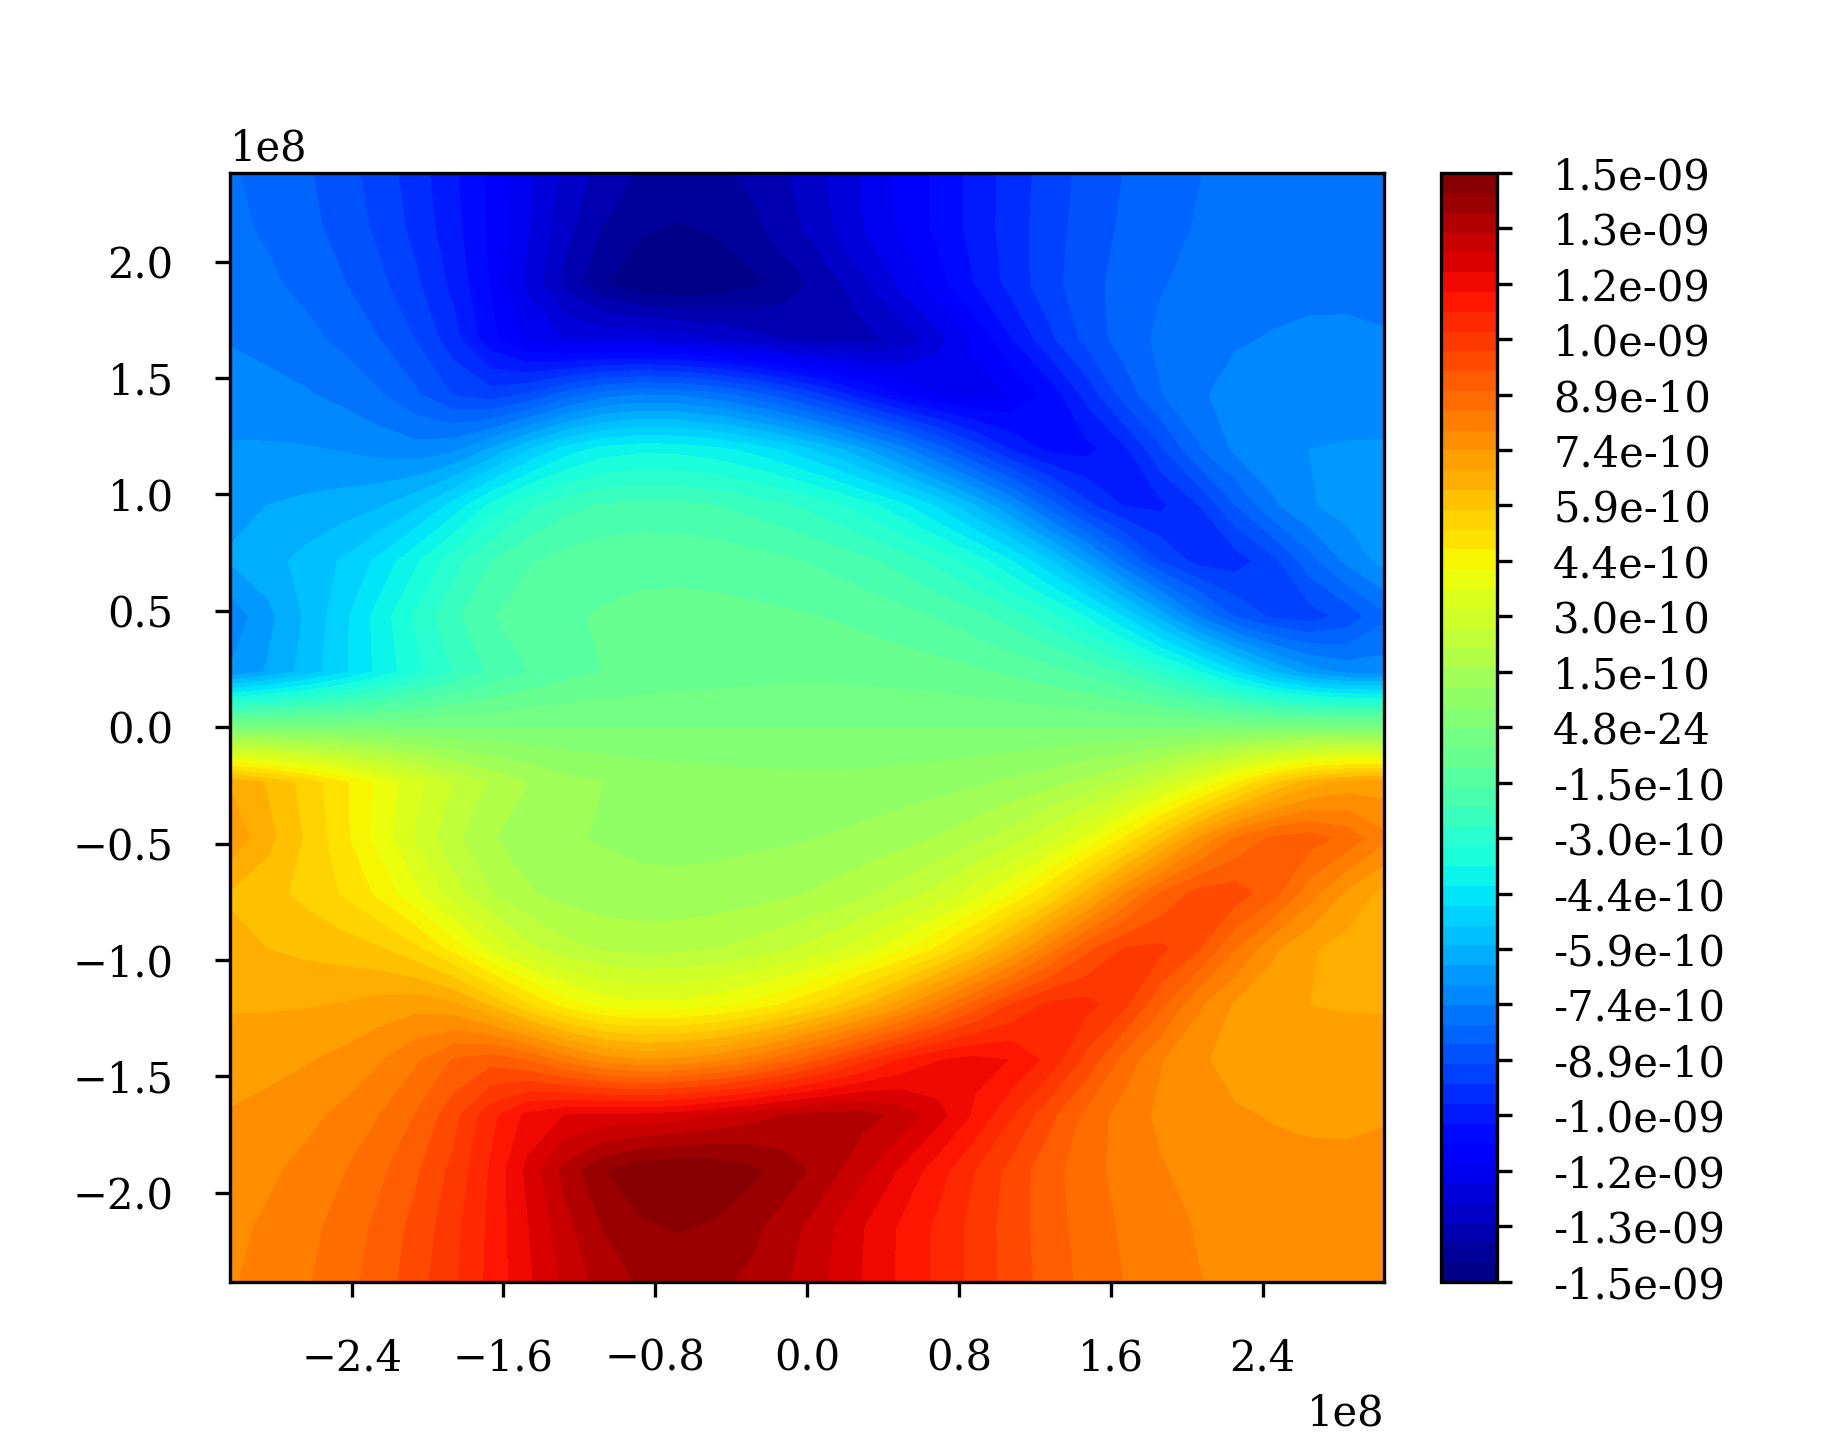
\includegraphics[width=\linewidth]{images/Bx_XYcut_e10.png}
	\caption{$\eta = 10^{10}$}
	\label{fig:Bx10}
\end{subfigure}
\begin{subfigure}{0.49\textwidth}
	\centering
	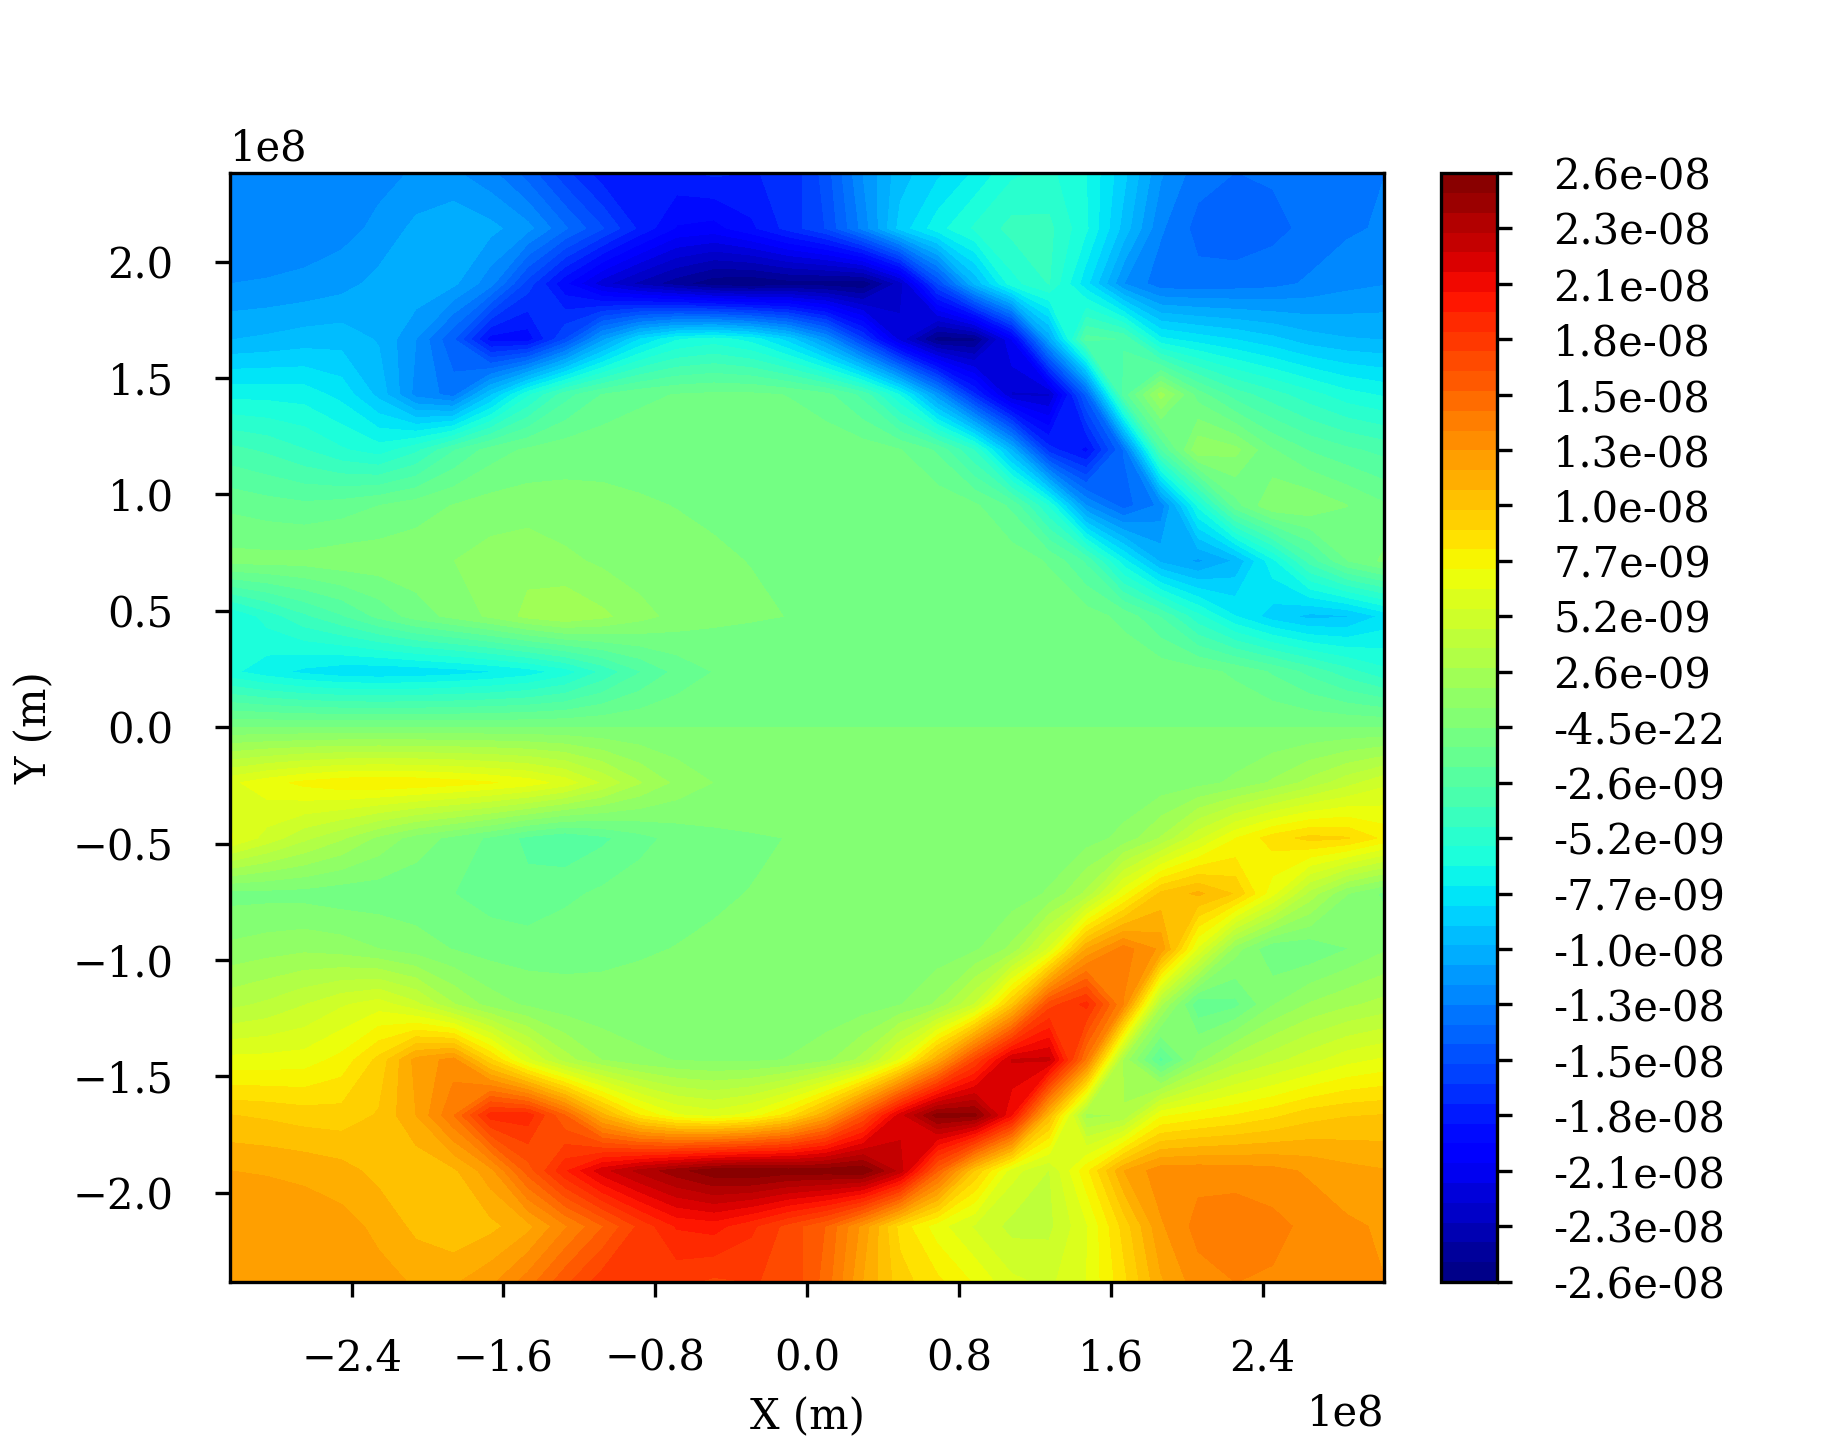
\includegraphics[width=\linewidth]{images/bx_05e7_500.png}
	\caption{$\eta = 10^8$}
	\label{fig:Bx8}
\end{subfigure}
\label{fig:Bx}
\caption{Z-averaged of $B_x$ in which $\eta=10^{10}$ (\ref{fig:Bx10}) and $\eta=10^{8}$ (\ref{fig:Bx8}). The snapshot is taken at 127 days and 500 days respectively.}
\end{figure}

\begin{figure}
\centering
\begin{subfigure}{0.49\textwidth}
\centering
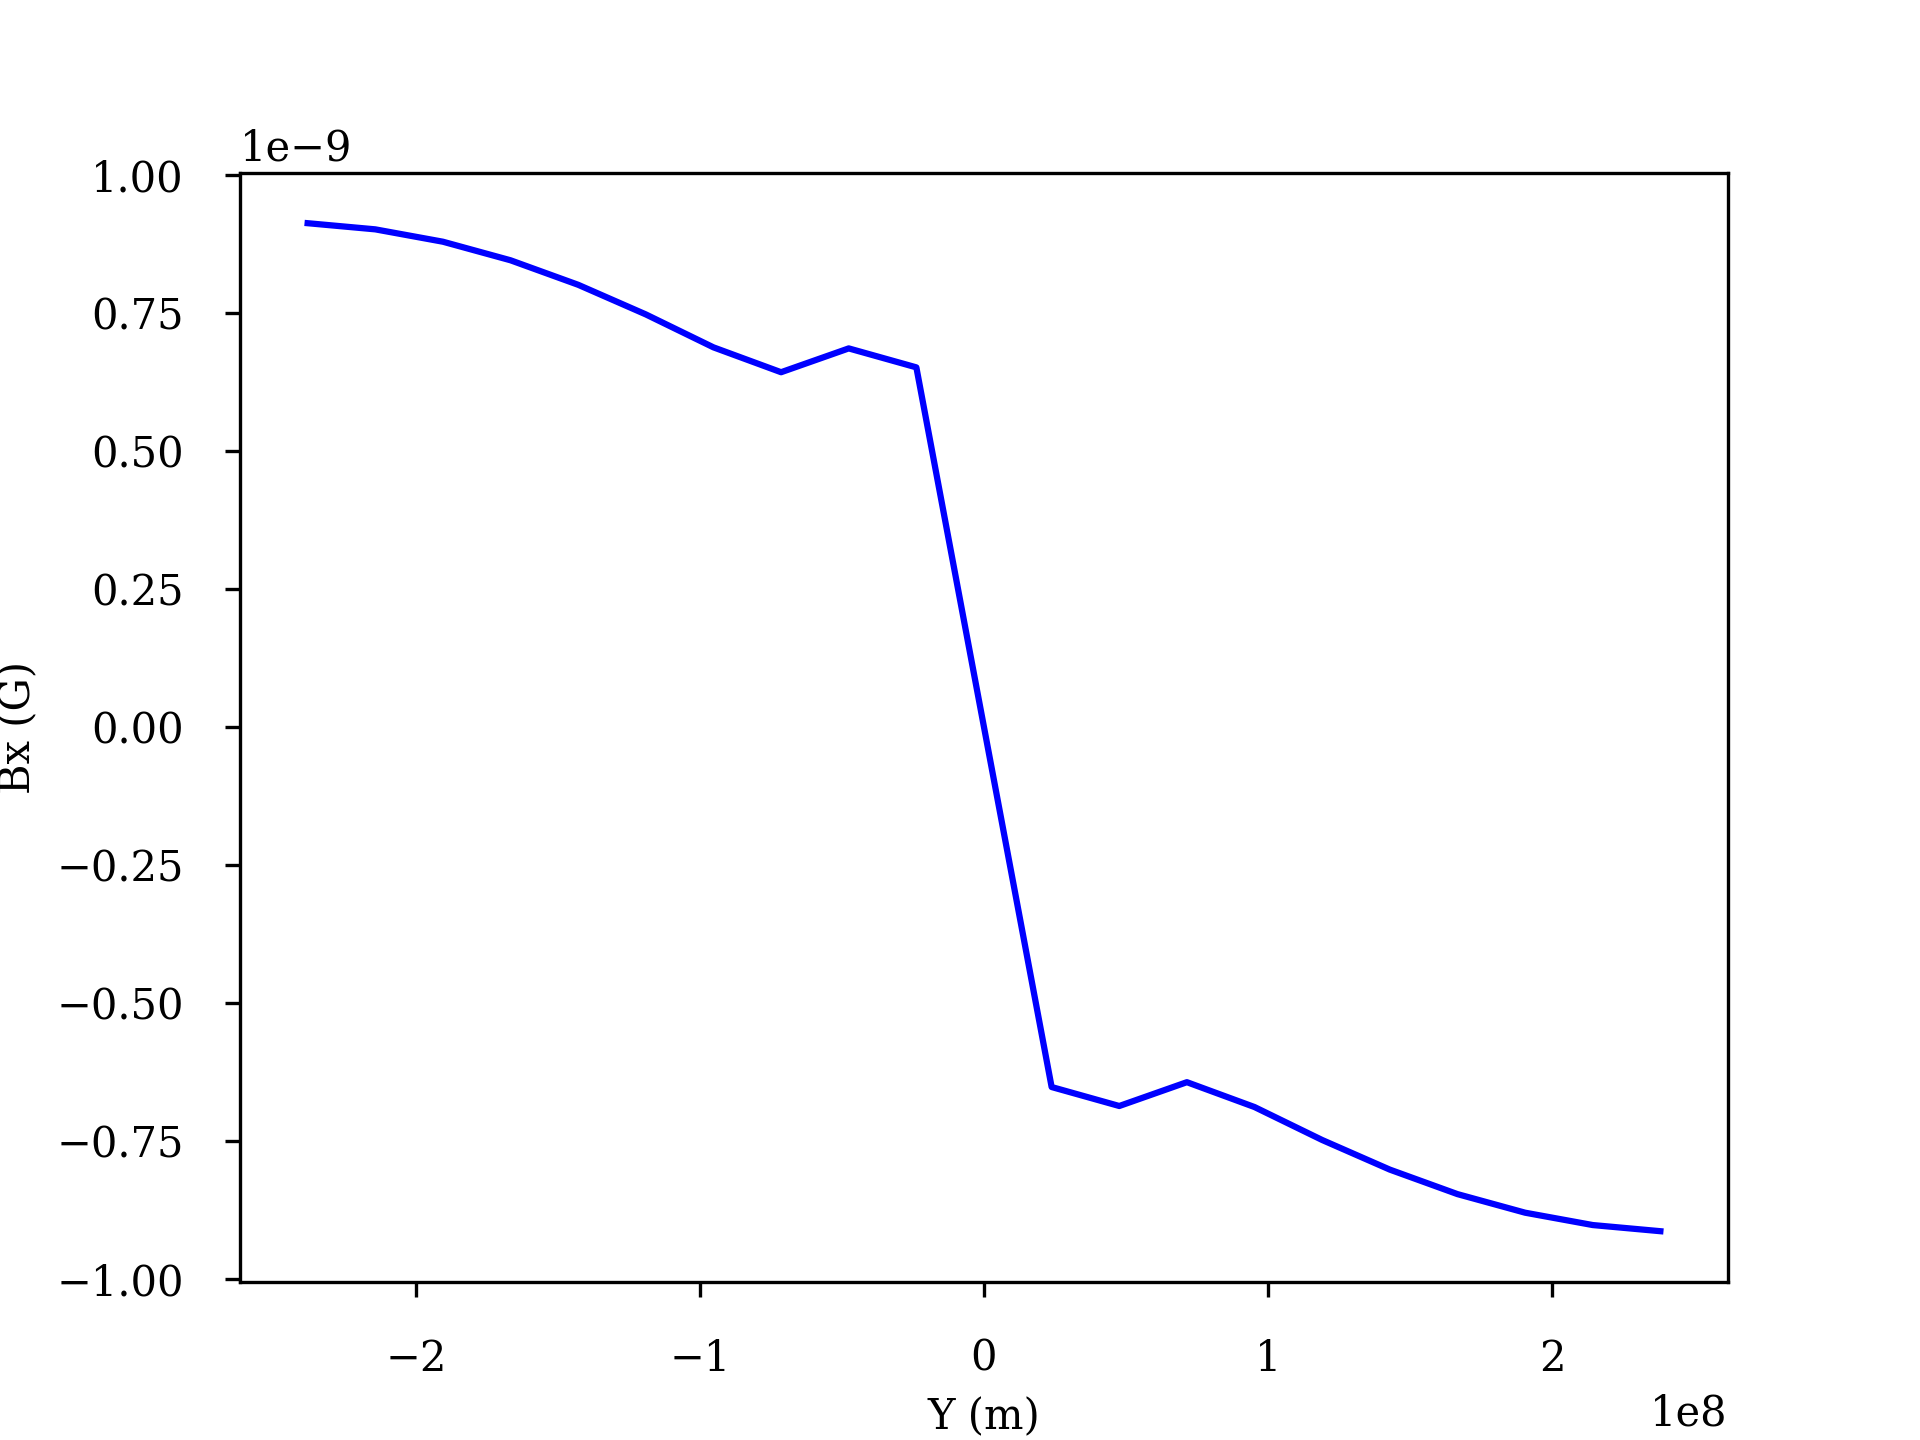
\includegraphics[width=\textwidth]{images/Bx_z1.png}
\caption{numerical $B_x$}
\label{fig:numBx}
\end{subfigure}
\begin{subfigure}{0.45\textwidth}
\centering
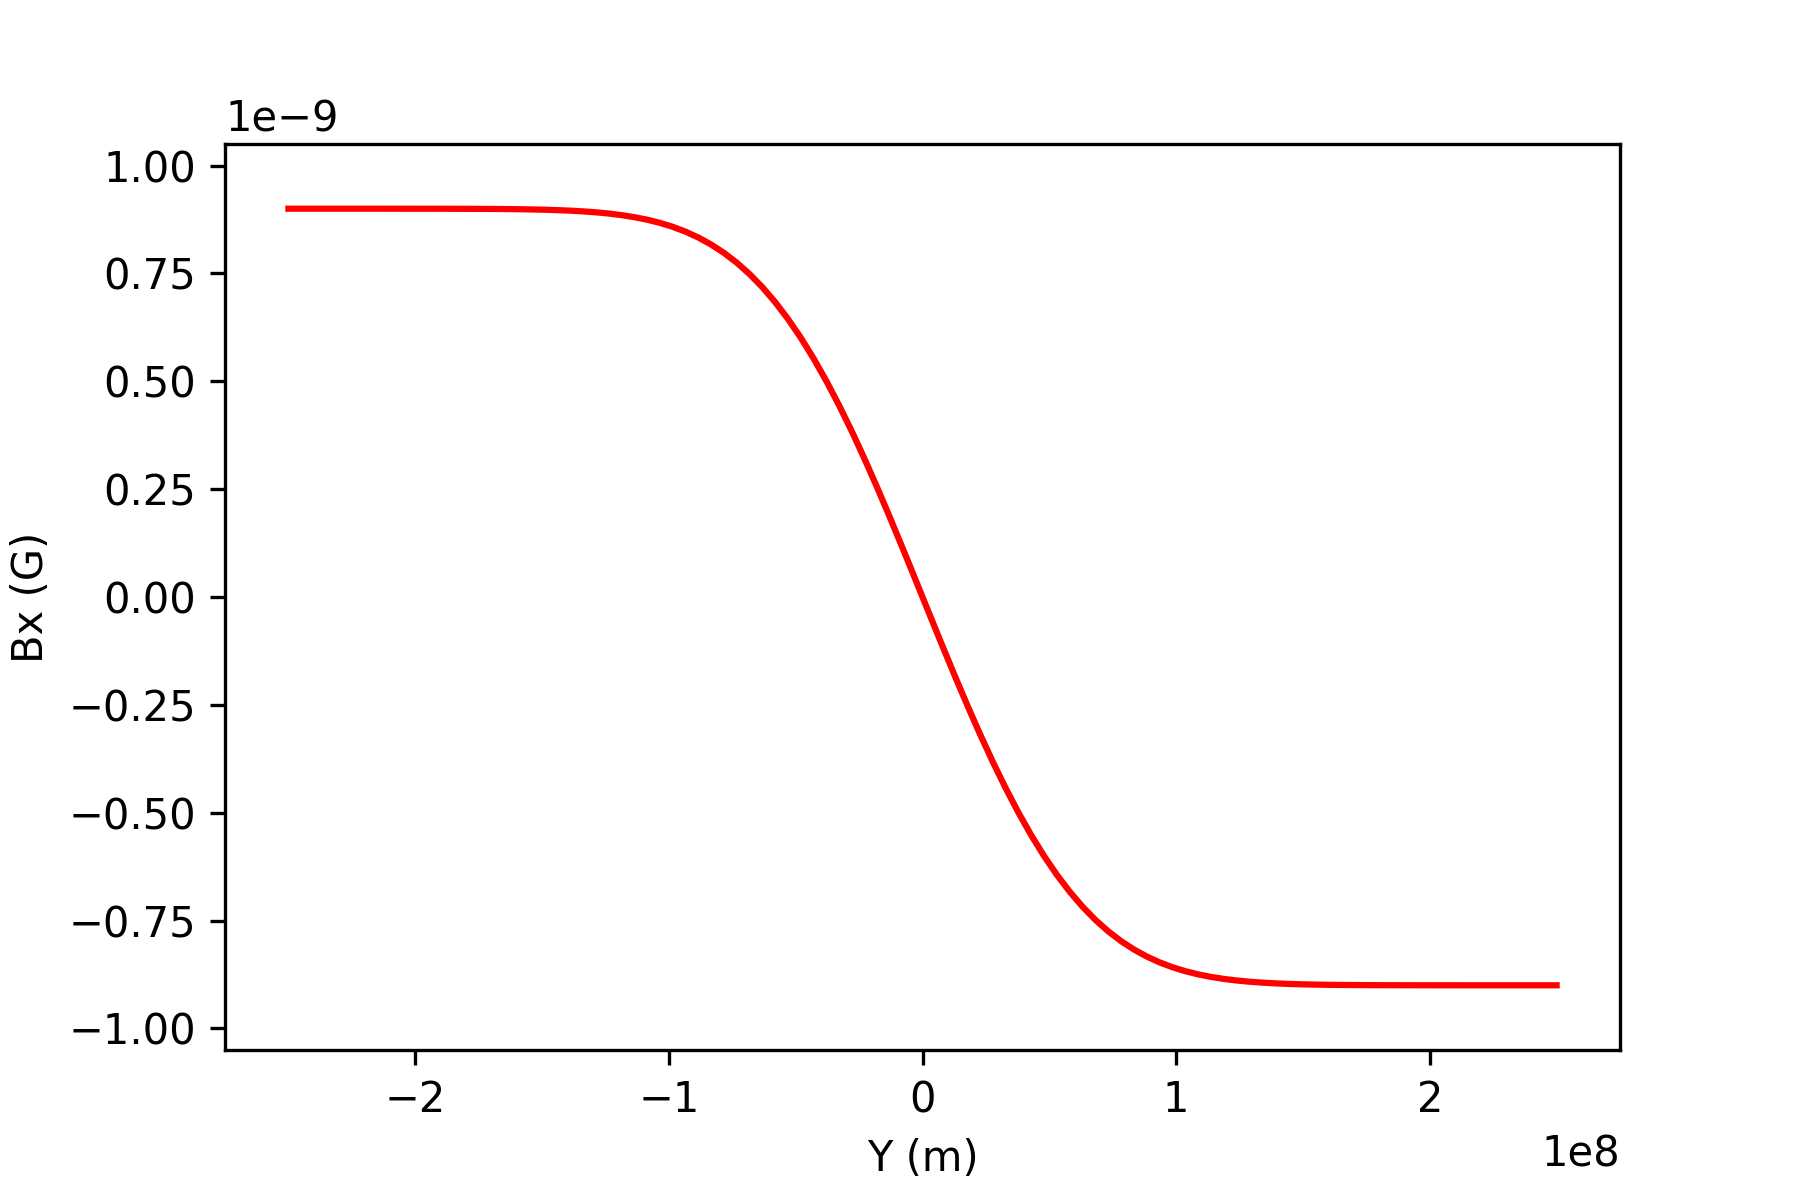
\includegraphics[ width=\textwidth , height = 6.1 cm  ]{images/Bx_ana.png}
\caption{analytical $B_x$}
\label{fig:anaBx}
\end{subfigure}

\caption{Z-averaged of $B_x$ (in G) at line of longitude of $x = -2.4 \times 10^8 m$ in which $\eta=10^{10}$ (\ref{fig:numBx}) and analytical solution from the simple model (\ref{fig:anaBx}). The snapshot is taken at t = 127 days. }
\label{fig:Bx_z1}
\end{figure}


We ran the simulation with small initial magnetic field and large diffusitivity, $\eta = 10^{10} \ m^2\cdot s^{-1} $. With this value of $\eta$, following the argument made in sect. \ref{NaiveModel}, advection timescale and diffusion timescale are actually comparable. So this is not entirely in a diffusion regime, advection still have a considerable effect on $B_x$. The figure \ref{fig:Bx10} and figure (?) shows an agreement between the flow ($v_y$) and $B_x$. $V_y$ pushes $B_x$ away from the equator, which creates a distinct spade-like pattern. However,in the region around the line of longitude of $x = -2.4 \times 10^{8} m $, the magnitude of $v_y$ is one order smaller and diffusion thus dominates, which makes it suitable for testing our simple model. Figure \ref{fig:Bx_z1} show the agreement of $B_x$ between the simple model and the simulation. $B_x$ will be diffused away from the equator until the equilibrium is established by reconection. Apart from the small deviation due to advection that the naive model fails to capture, the analytical solution generally follows the numerical $B_x$. Besides, $B_x$ is 1 order larger than $B_0$ as expected.
\label{sec:eta10}
\subsection{Small magnetic field with $ \boldsymbol{\eta} = \boldsymbol{10^{8}} \ \boldsymbol{m^2 \cdot s^{-1}}$} 

\begin{figure}
\begin{subfigure}{0.49\textwidth}
	\centering
	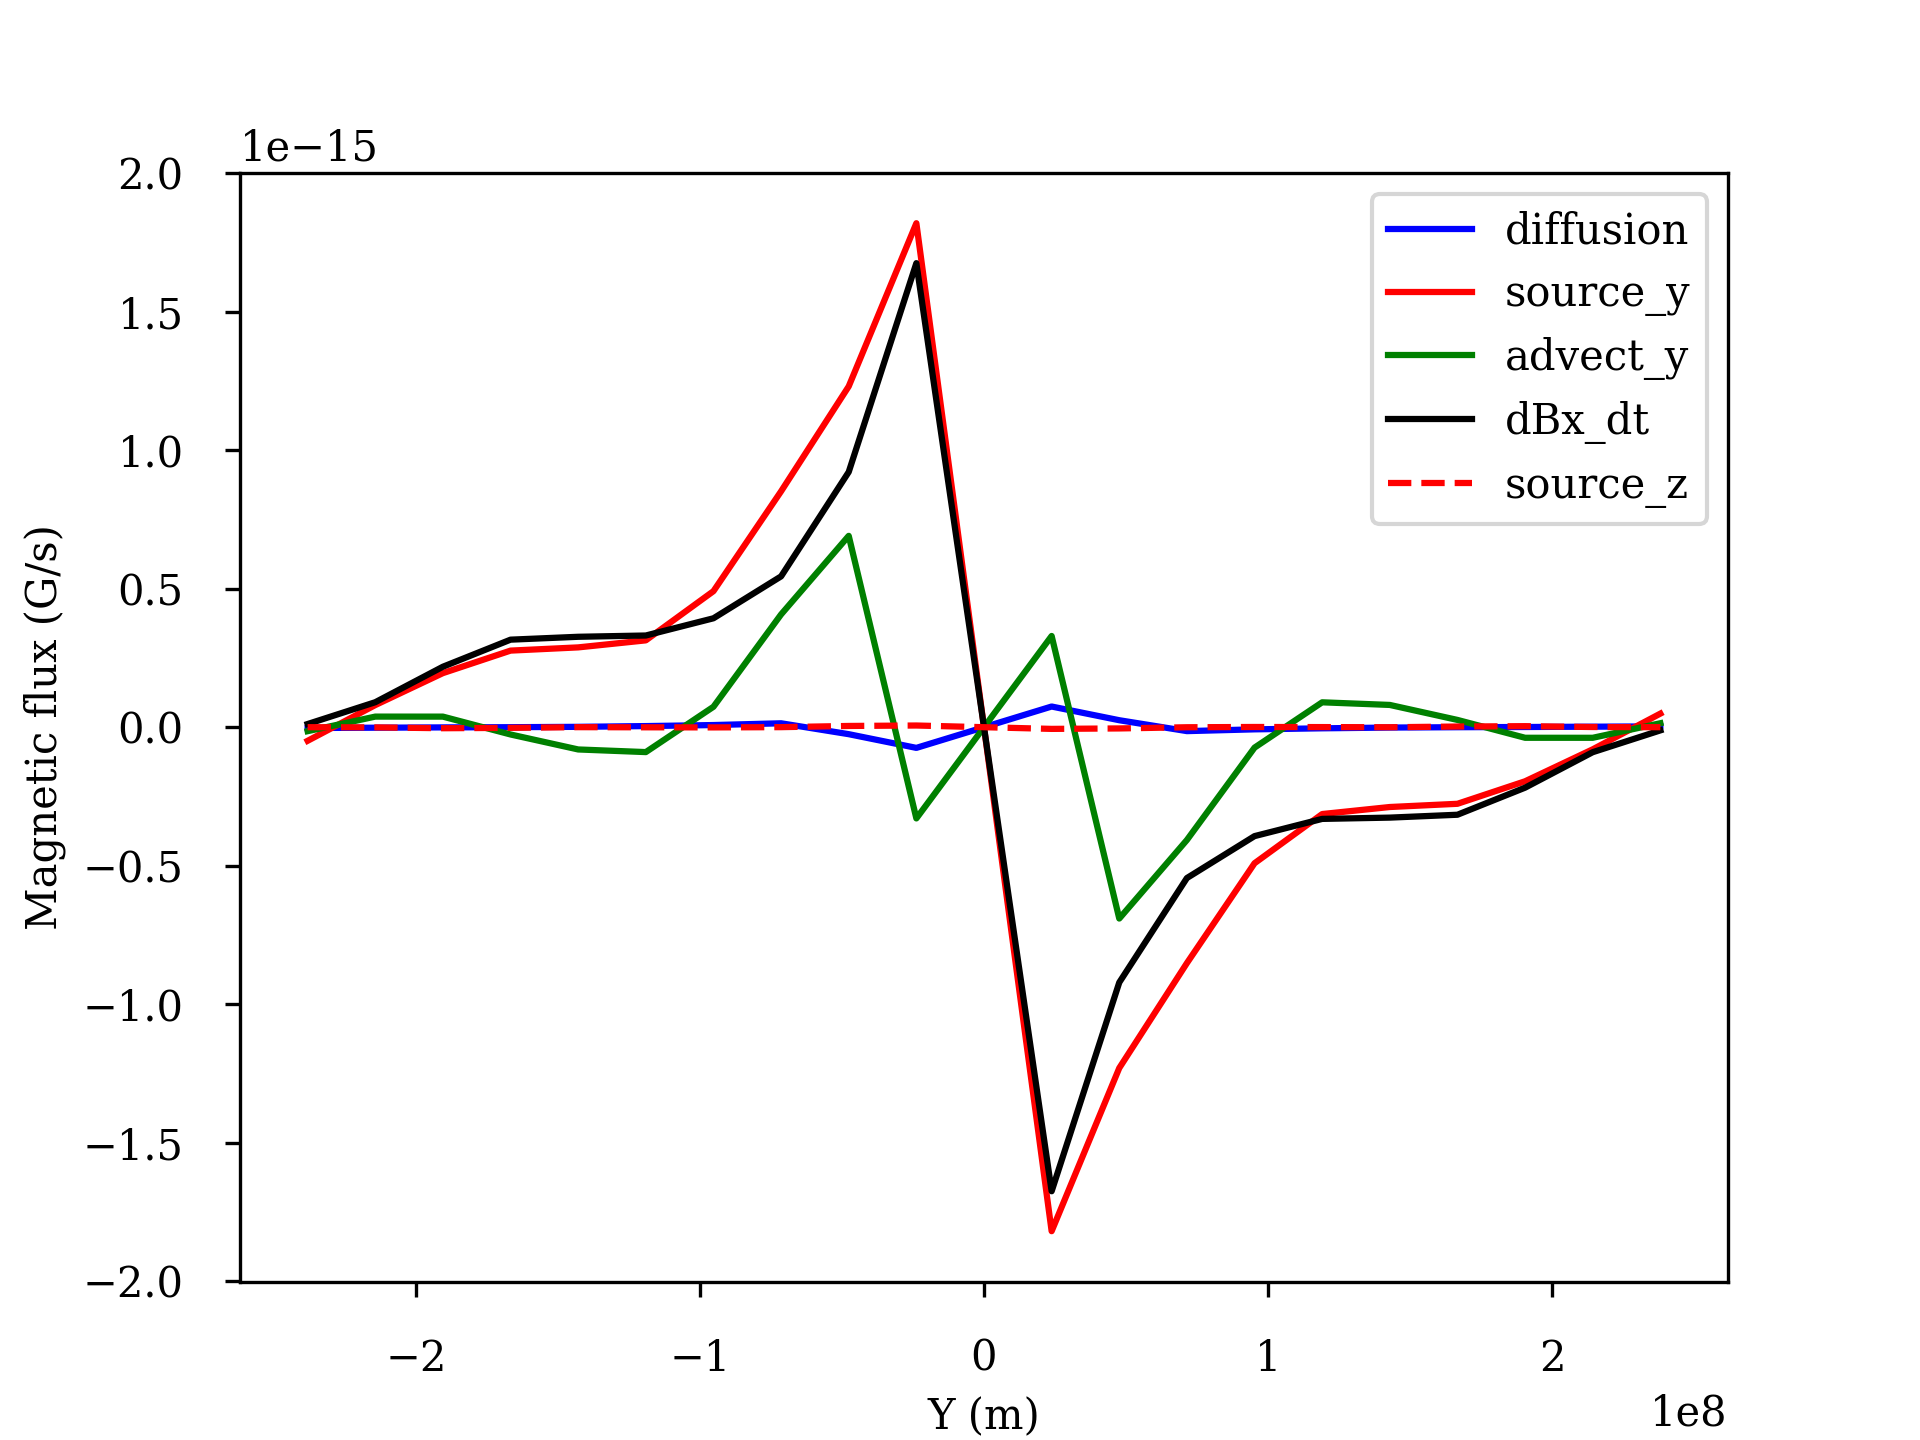
\includegraphics[width=\linewidth]{images/compare_YZaver_100_lg.png}
	\caption{$t = 100\ days$}
	\label{fig:Compare_t100}
\end{subfigure}
\begin{subfigure}{0.49\textwidth}
	\centering
	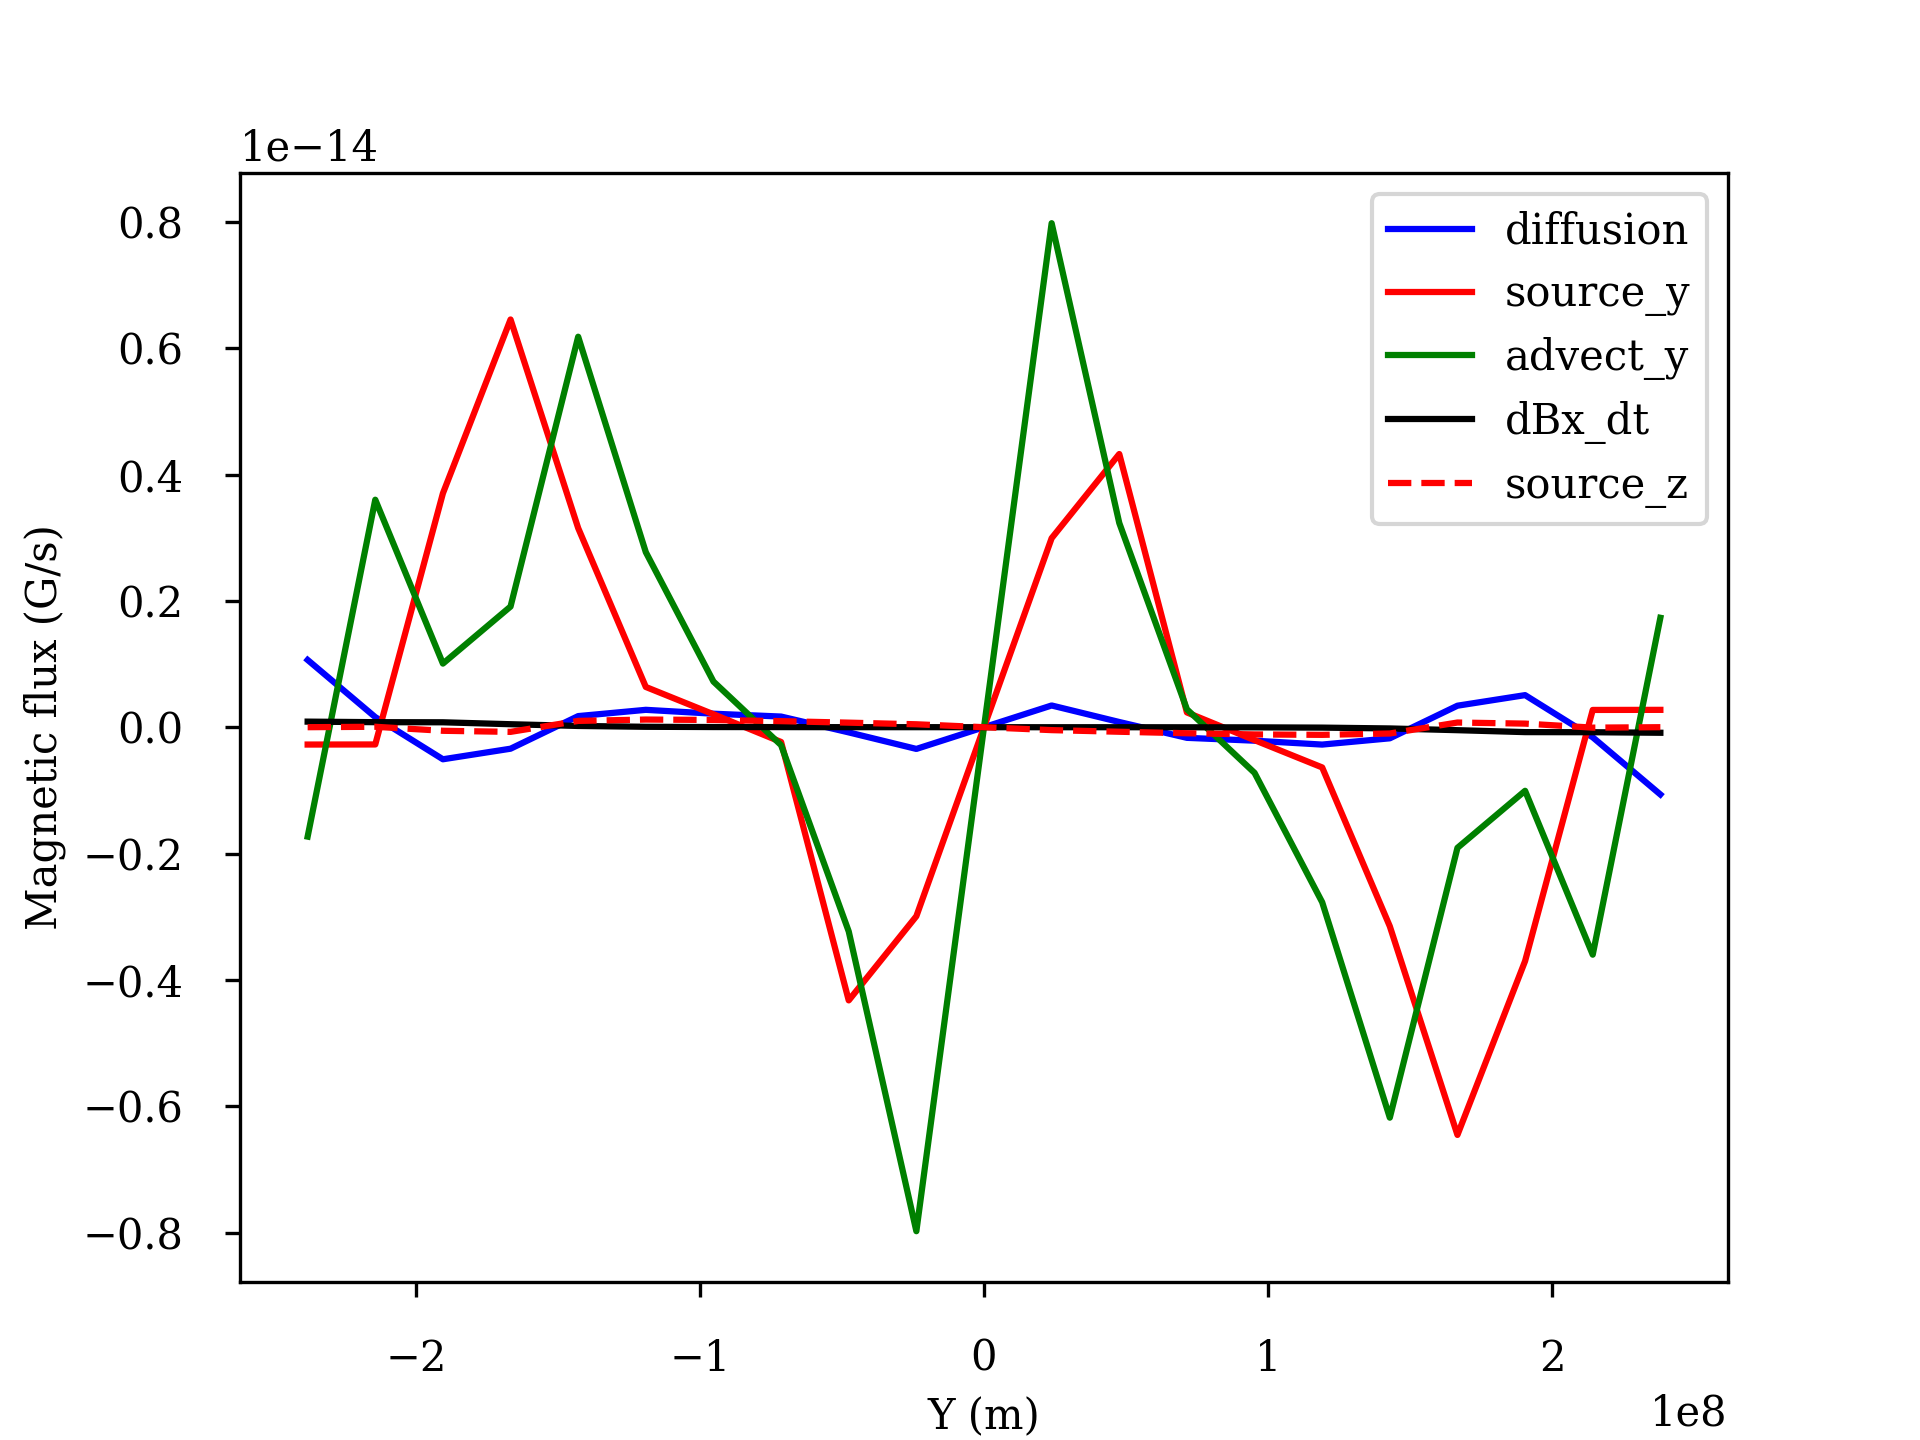
\includegraphics[width=\linewidth]{images/compare_YZaver_500_lg.png}
	\caption{$t = 500\ days$}
	\label{fig:Compare_t500}
\end{subfigure}
\caption{Zonally and vertically averaged of each term in equation \ref{eq:ind} initially (\ref{fig:Compare_t100}) and in steady state (\ref{fig:Compare_t500}). The snapshot is taken at 100 days and 500 days respectively.}
\label{fig:Compare}
\end{figure}
  
We ran this simulation with small magnetic field and small diffusitivity - $\eta = 10^{8} \ m^2 \cdot s^{-1}$. In y direction, following the argument of order made in section \ref{NaiveModel}, this case is in advection regime, namely the flow dictates the structure of $B_x$ horizontally. 

Figure (\ref{fig:Bx8}) and figure (?) show the strong correlation between $B_x$ and $v_y$, which is the evidence for the strong effect of the advection on the magnetic field. The longitudinal velocity seems to bring $B_x$ to where it halts. But upon closer inspection at contribution of each term in eq. (\ref{eq:ind}) in figure(\ref{fig:Compare}), especially when it reaches steady state, we see that the source - the stretching terms at the sides are actually stronger than the source in the middle. And the source in the middle interestingly reverses side. Nevertheless, because of the strong longitude-dependence of the variables, xy-plot should be refered. 

Figure (\ref{fig:By}) depitcts $B_y$ in steady state, which is developed at the sides due to the stretching of $B_x$ by $v_y$. The pattern of $B_y$ creates the parities of adjoining source-sink (figure \ref{fig:source500}) Advection helps to bring these to reconnection, which renders the system into steady state figure(\ref{fig:advect}). So, contrary to the high $\eta$ case (sect. \ref{sec:eta10}), in which diffusion is the driving force, advection is apparently the one in this case.
\begin{figure}
\begin{subfigure}{0.49\textwidth}
	\centering
	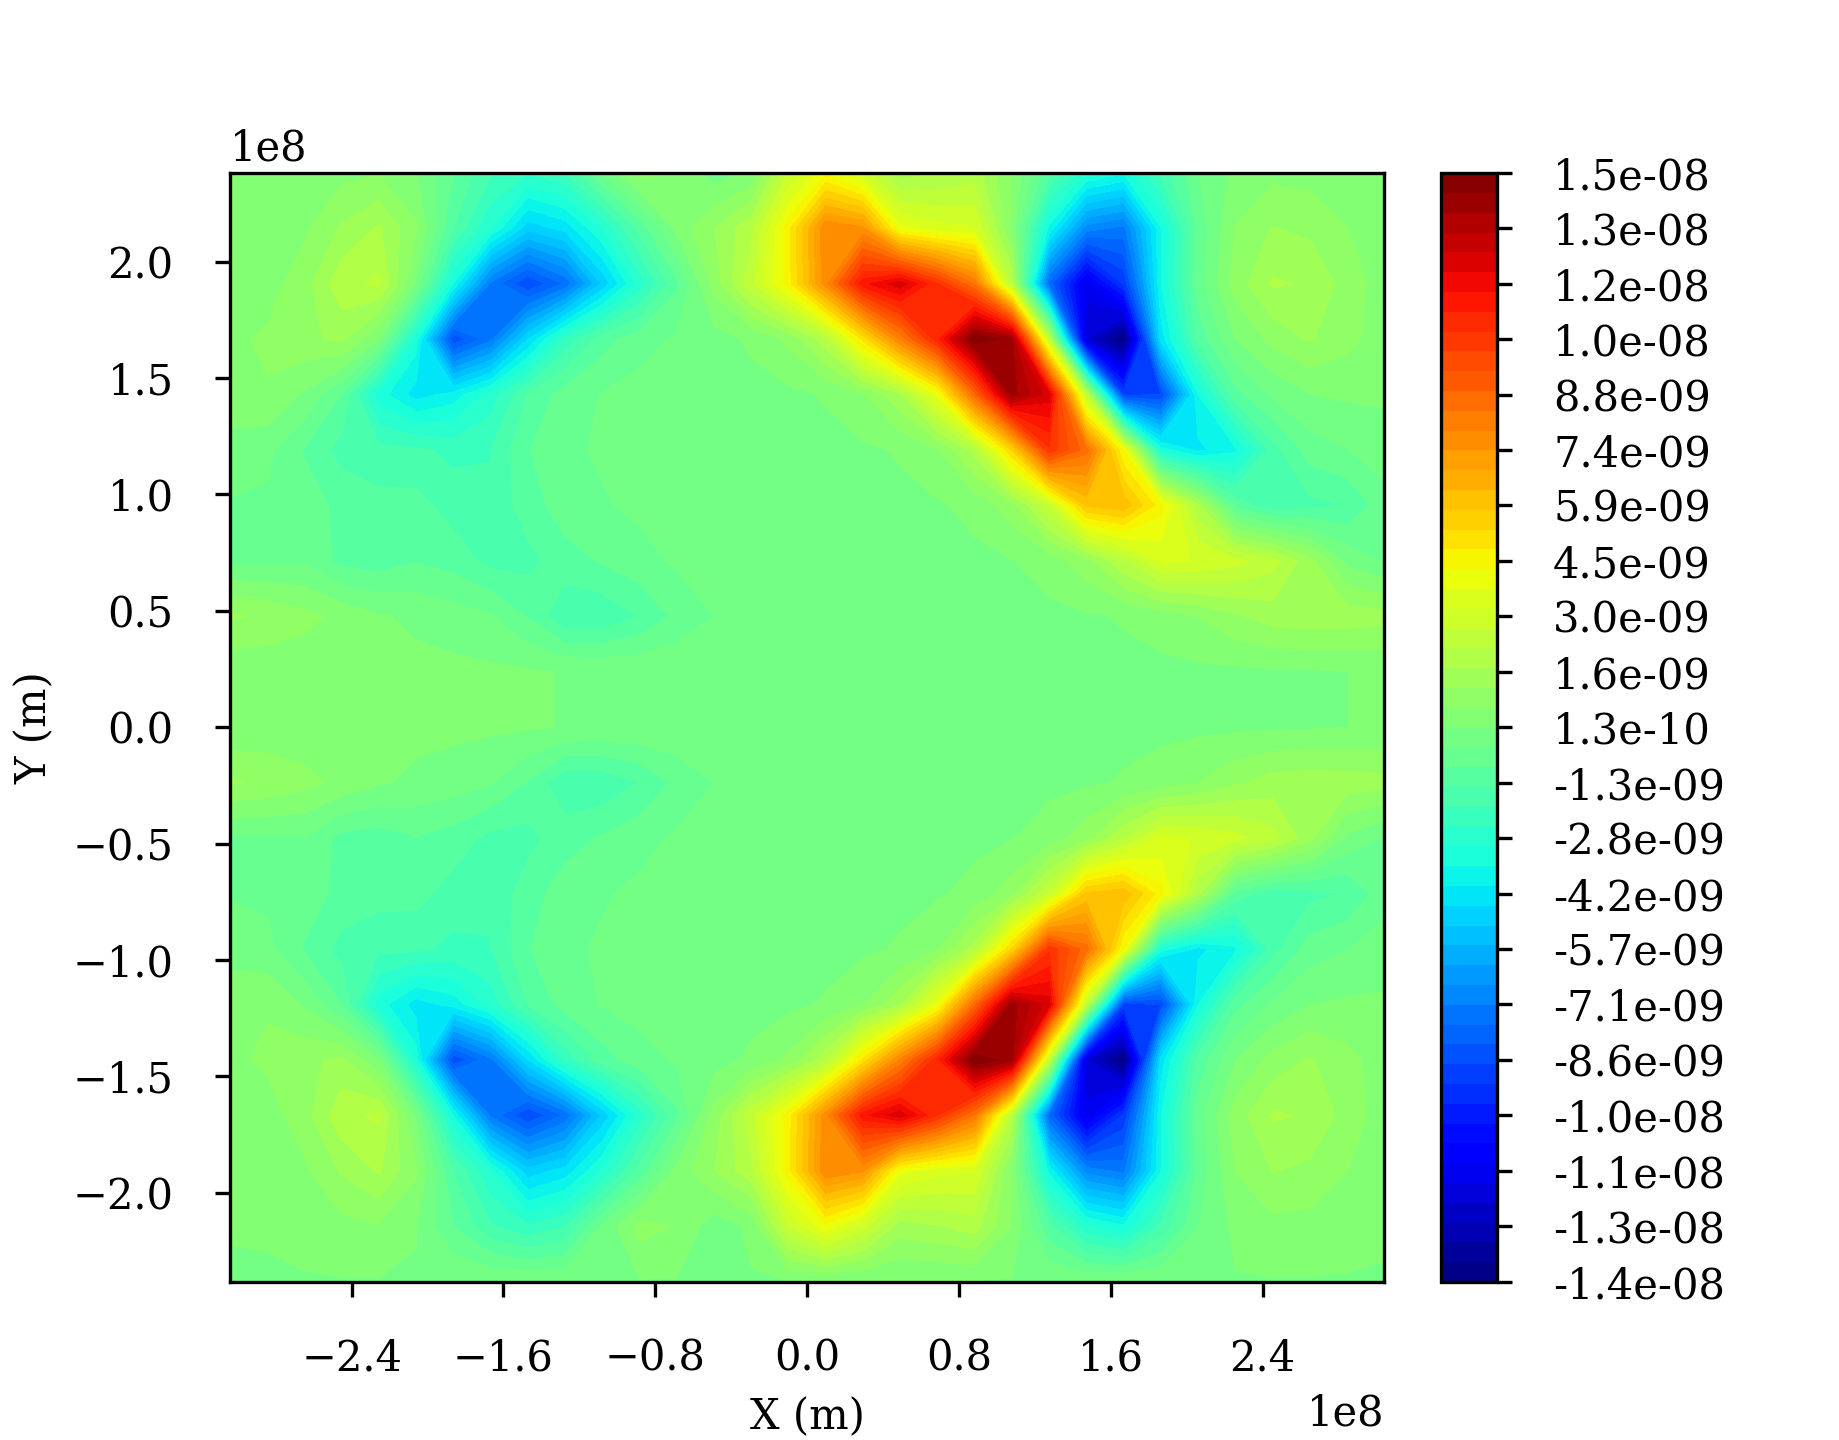
\includegraphics[width=\linewidth]{images/by_05e7_500.png}
	\caption{}
	\label{fig:By}
\end{subfigure}
\begin{subfigure}{0.49\textwidth}
	\centering
	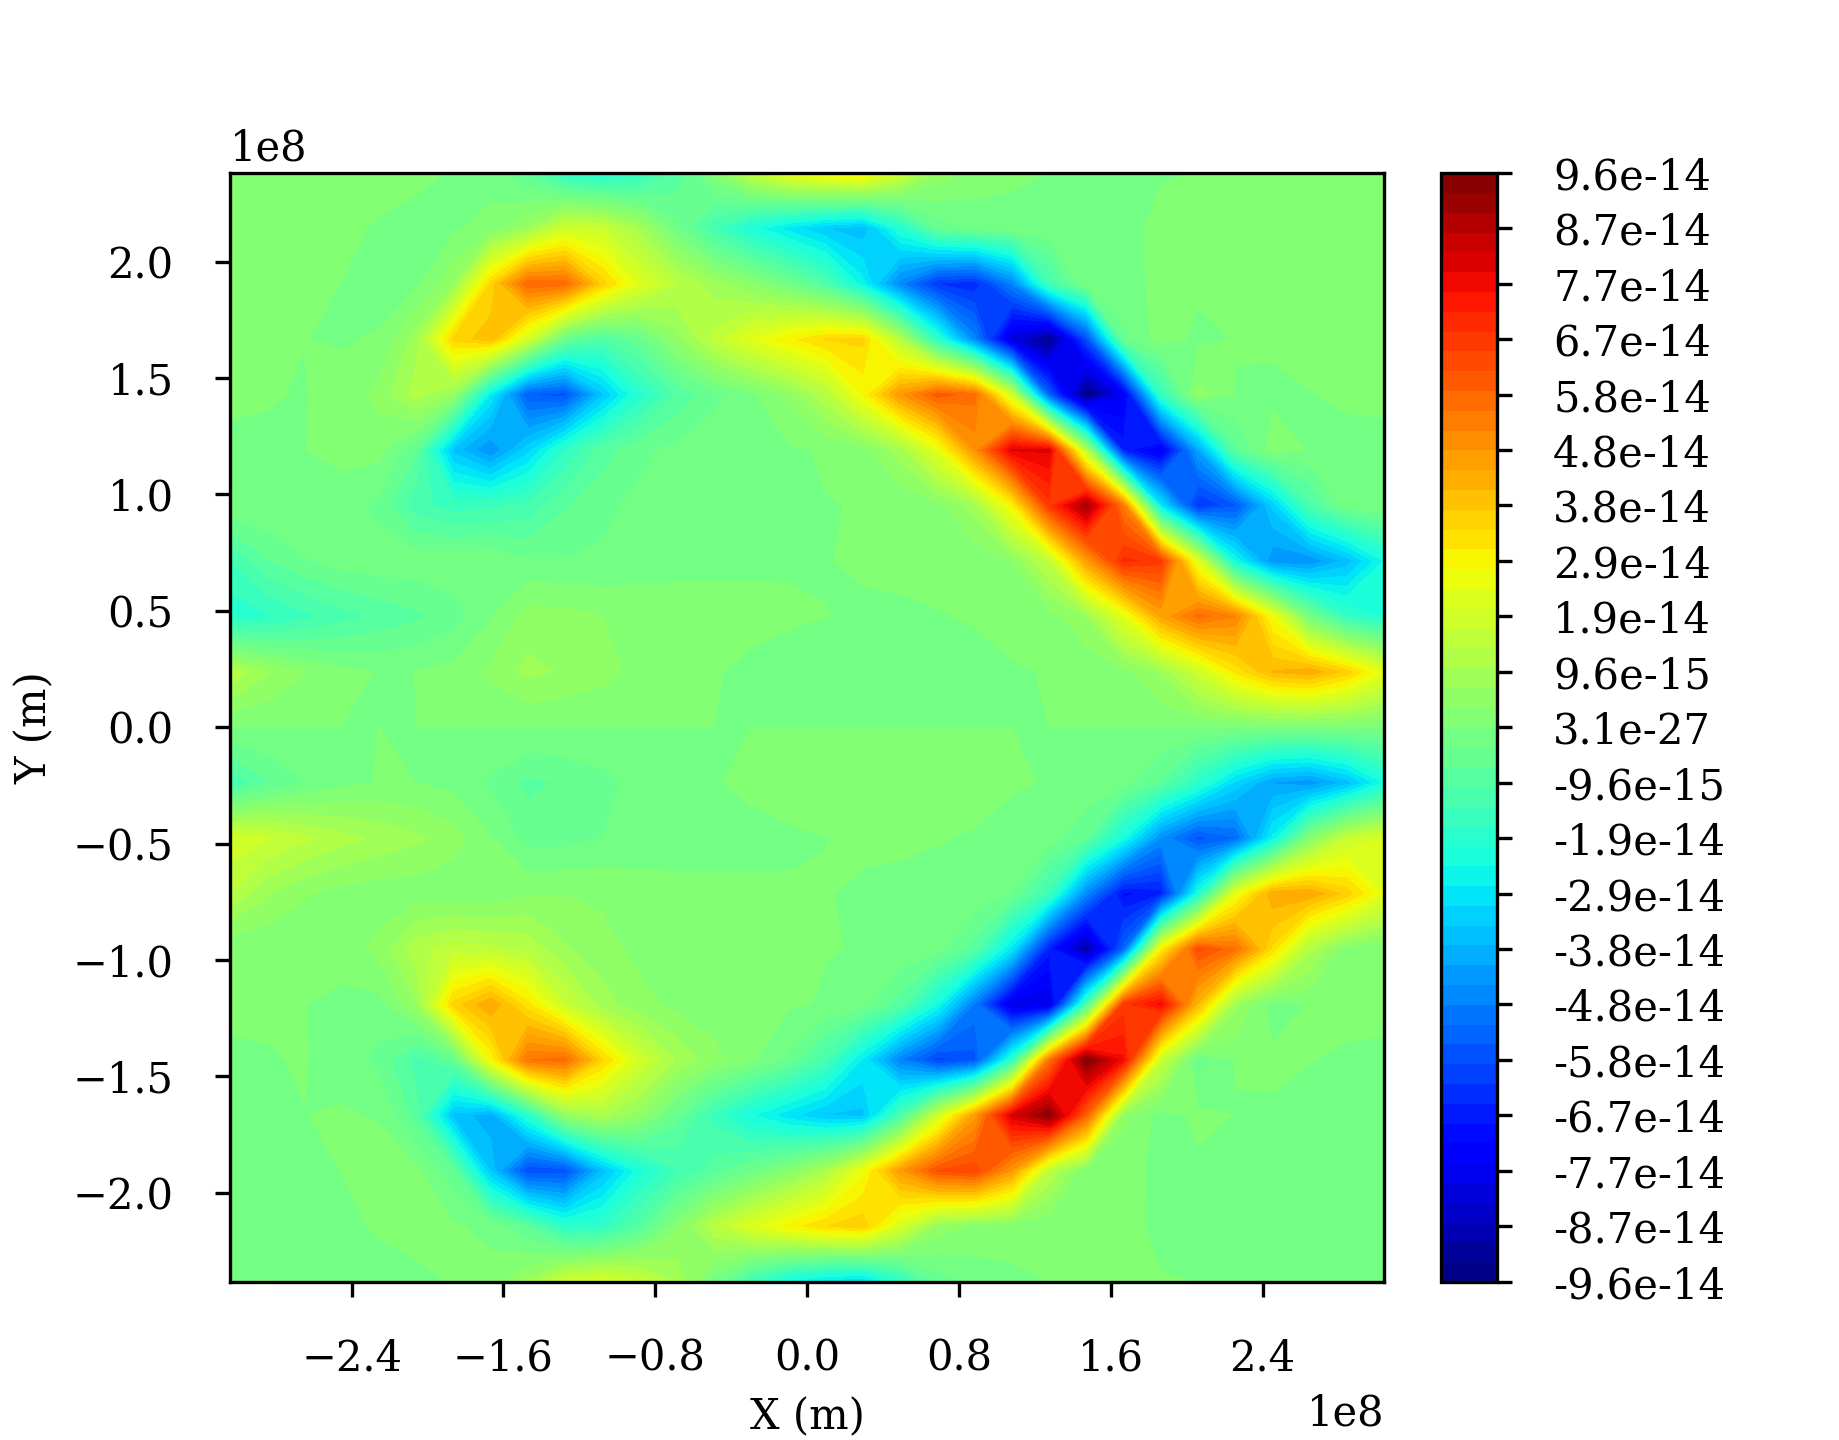
\includegraphics[width=\linewidth]{images/advect_aver_500.png}
	\caption{}
	\label{fig:advect}
\end{subfigure}

\begin{subfigure}{0.49\textwidth}
	\centering
	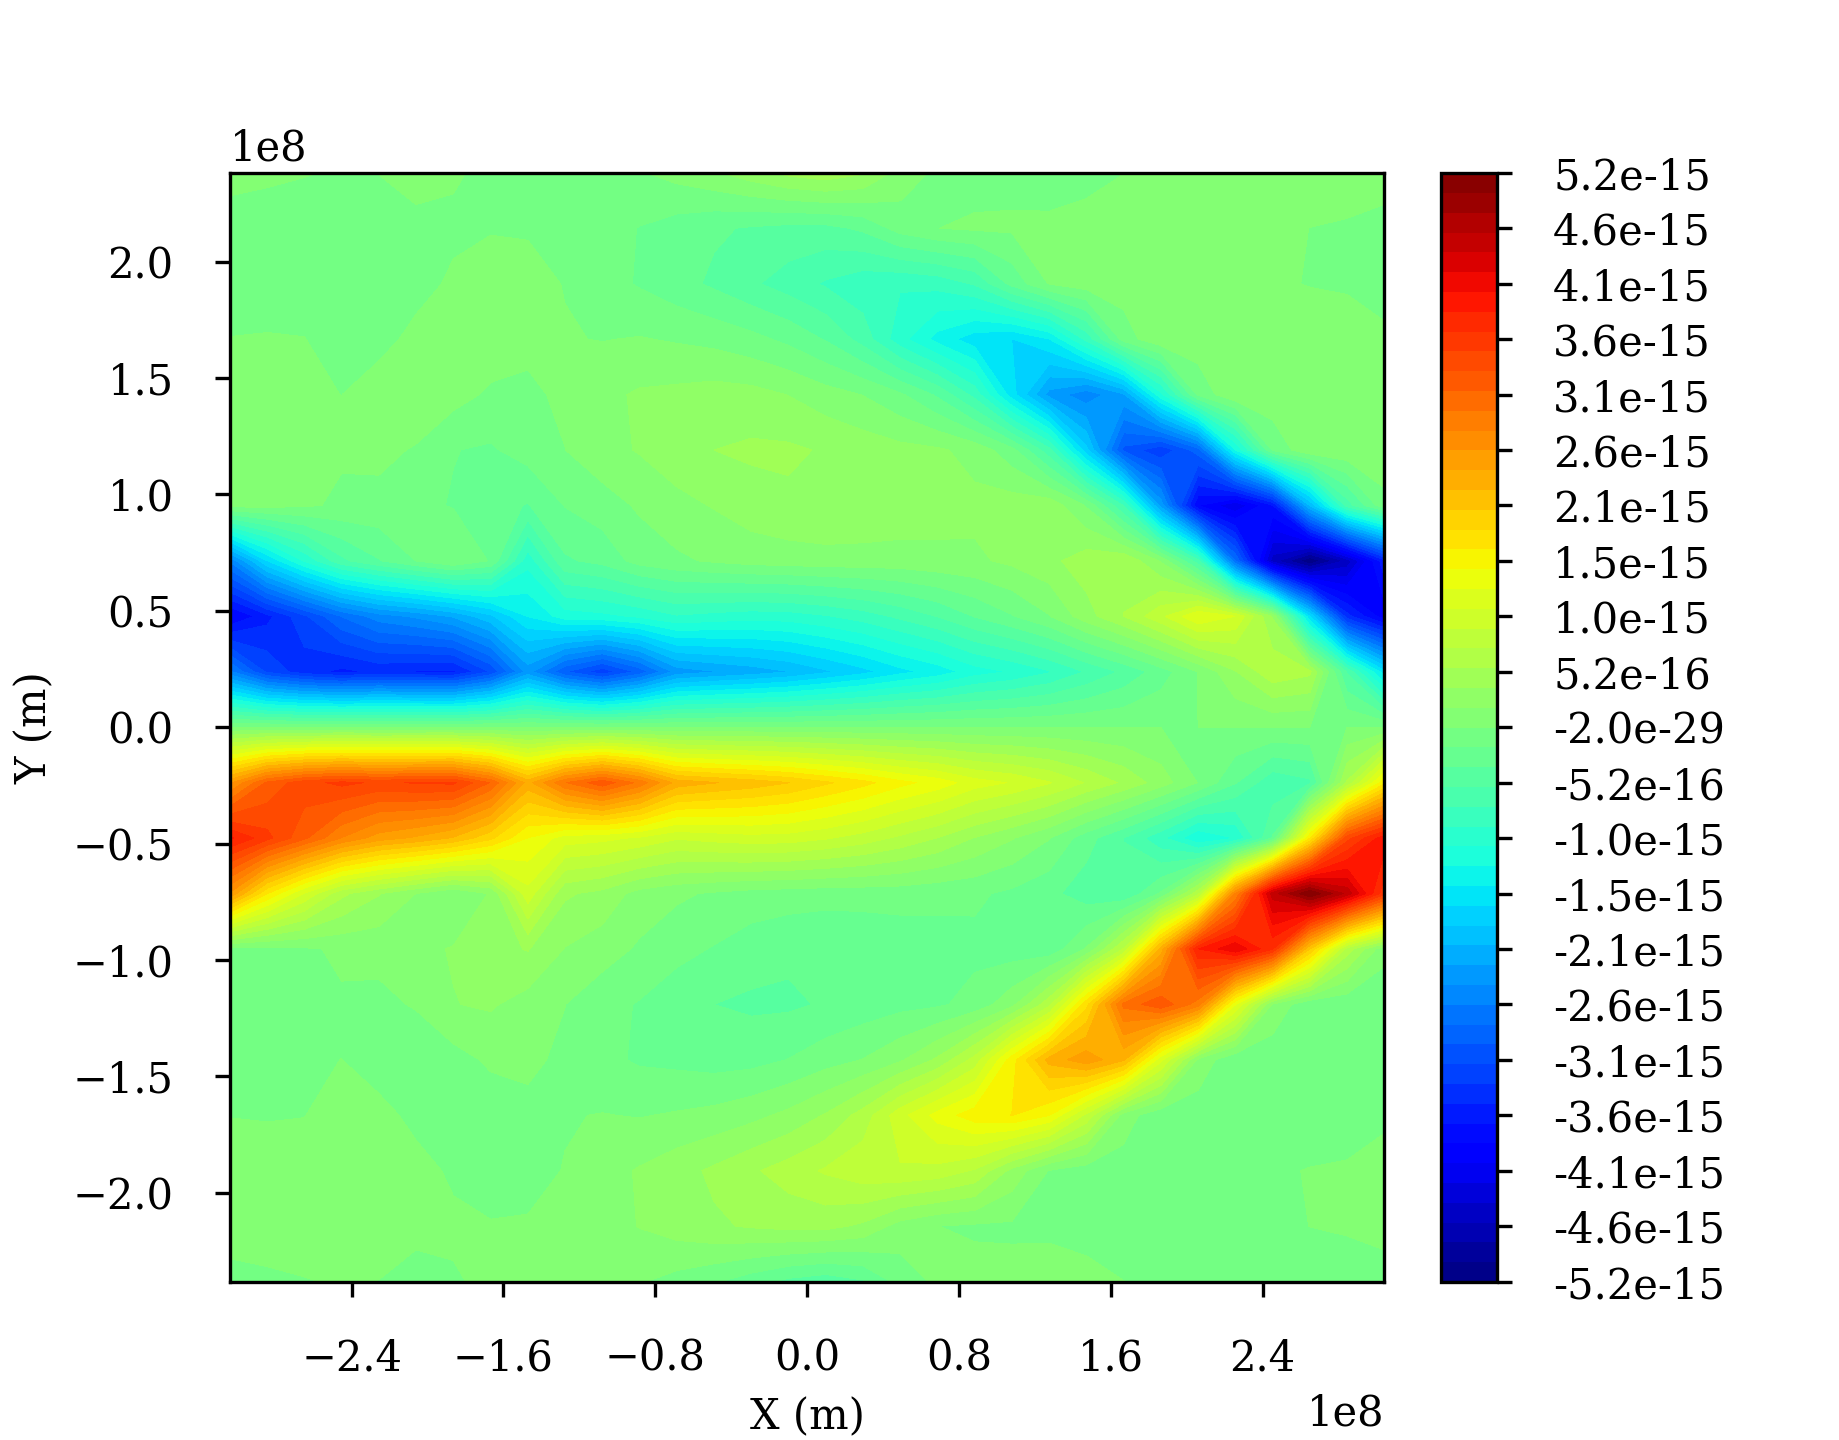
\includegraphics[width=\linewidth]{images/source_aver_100.png}
	\caption{}
	\label{fig:source100}
\end{subfigure}
\begin{subfigure}{0.49\textwidth}
	\centering
	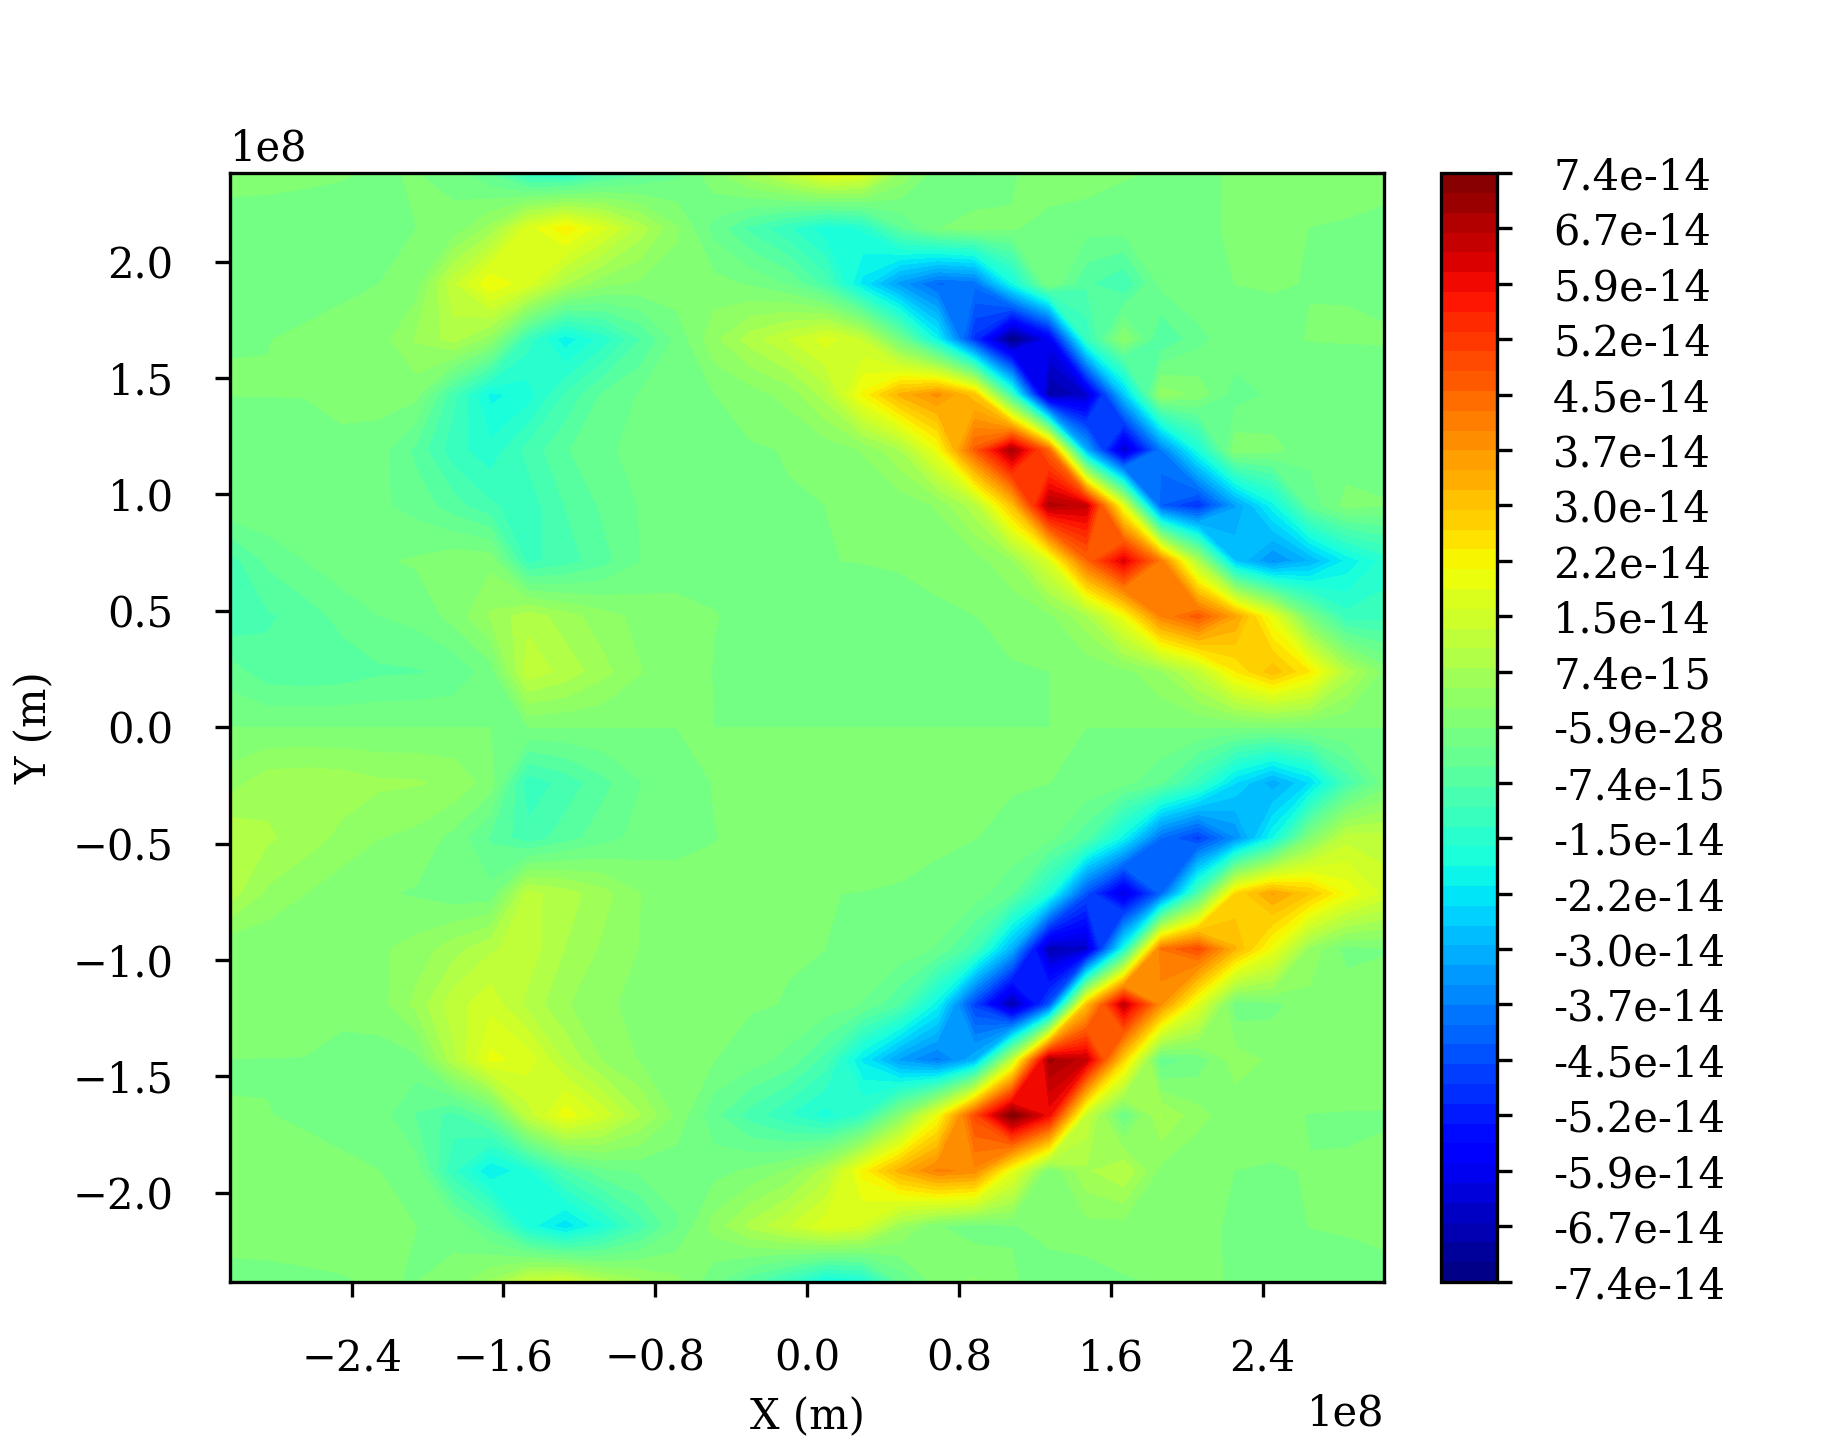
\includegraphics[width=\linewidth]{images/source_aver_500.png}
	\caption{}
	\label{fig:source500}
\end{subfigure}
\caption{Color contour plots show the vertically-averaged of the variables: $B_y$ in G (\ref{fig:By}); advection term in in G/s (\ref{fig:advect}); source term in G/s (\ref{fig:source100},\ref{fig:source500}. The snapshot is taken initially at 100 days (c) and in steady state at 500 days(a,b,d).}
\label{fig:Misc}
\end{figure}
%
%\begin{figure}
%\centering
%\begin{subfigure}
%\includegraphics[scale=•]{•}

\section{Discussion}
\subsection{D1}
\subsection{D2}

\bibliography{reference}

\end{document}

%The structure of the magnetic field is determined by the place where movement is strongest
